
%设置幻灯片格式为16:9
% \documentclass[aspectratio=169]{beamer}
% 幻灯片格式4:3
\documentclass[aspectratio=169]{beamer}
\usepackage[BoldFont,SlantFont]{xeCJK}
\setCJKmainfont[Path=fonts/]{STKAITI.TTF}
\setCJKsansfont[Path=fonts/]{STKAITI.TTF}
\setCJKmonofont[Path=fonts/]{STKAITI.TTF}
\setmainfont{Times New Roman}
\setsansfont{Times New Roman}
\setmonofont{Times New Roman}
\usepackage{fontenc}
\usepackage{hyperref}
\usepackage{subcaption}
% other packages
\usepackage{latexsym,amsmath,xcolor,multicol,booktabs,calligra}
\usepackage{graphicx,pstricks,listings,stackengine}

\usepackage[numbers, sort&compress]{natbib}
\bibliographystyle{plainnat}


\usepackage{bm}
\usepackage{amssymb}
\usepackage{multirow}
\usefonttheme{serif}
\setbeamertemplate{navigation symbols}{}
\usepackage{caption}
\captionsetup{font={scriptsize}}
% \author{王国康  云鑫  杨艺辉}
\author{WangGuokang YunXin YangYihui}
% \author[a]{王国康}
% \author[b]{云鑫}
% \author[c]{杨艺辉}
\title{Professional English 2025 Presentation}
\subtitle{From Speaker to Dubber: Movie Dubbing with
Prosody and Duration Consistency Learning}
\institute{School of Computer Science and Technology in USTC}
\date{2025年4月25日}
\usepackage{ustc}


% defs
\def\cmd#1{\texttt{\color{red}\footnotesize $\backslash$#1}}
\def\env#1{\texttt{\color{blue}\footnotesize #1}}
\definecolor{deepblue}{rgb}{0,0,0.5}
\definecolor{deepred}{rgb}{0.6,0,0}
\definecolor{deepgreen}{rgb}{0,0.5,0}
\definecolor{halfgray}{gray}{0.55}

\lstset{
    basicstyle=\ttfamily\small,
    keywordstyle=\bfseries\color{deepblue},
    emphstyle=\ttfamily\color{deepred},    % Custom highlighting style
    stringstyle=\color{deepgreen},
    numbers=left,
    numberstyle=\small\color{halfgray},
    rulesepcolor=\color{red!20!green!20!blue!20},
    frame=shadowbox,
}

\setbeamertemplate{caption}[numbered]
\renewcommand\figurename{Figure} 
\renewcommand\tablename{Table}

\usepackage{perpage} %the perpage package
\MakePerPage{footnote} %the perpage package command

\newfontfamily\wingdingfamily[Path=fonts/]{wingding.ttf}
\newcommand\headtoright{%
  \texorpdfstring{{\wingdingfamily\XeTeXglyph190\relax}}{???}}

\setbeamertemplate{itemize item}{\headtoright}
\setbeamertemplate{itemize subitem}{$\bullet$}
\setbeamertemplate{itemize subsubitem}{$\circ$}


\begin{document}

\begin{frame}
    \titlepage
    \begin{figure}[htpb]
        \begin{center}
            
\includegraphics[width=0.2\linewidth]{figs/ustc_logo.pdf}
        \end{center}
    \end{figure}
\end{frame}

% ppt的介绍也目录设置
\begin{frame}
    \frametitle{Outline}
    \begin{columns}[T] % 对齐方式:顶部对齐
        \begin{column}{0.48\textwidth}
            \large
            \tableofcontents[sections={1-4}, sectionstyle=show, subsectionstyle=show/shaded/hide, subsubsectionstyle=show/shaded/hide]
        \end{column}
        \begin{column}{0.48\textwidth}
            \large
            \tableofcontents[sections={5-}, sectionstyle=show, subsectionstyle=show/shaded/hide, subsubsectionstyle=show/shaded/hide]
        \end{column}
    \end{columns}
\end{frame}

% \section{课题背景}

\begin{frame}{用Beamer很高大上?}
    \begin{itemize}[<+-| alert@+>] % 当然,除了alert,手动在里面插 \pause 也行
        \item 大家都会\LaTeX{},好多学校都有自己的Beamer主题
        \item 中文支持请选择 Xe\LaTeX{} 编译选项
        \item GitHub项目地址位于 \url{https://github.com/yangyihui2020/ustc_beamer_theme}
    \end{itemize}
\end{frame}

% \section{研究现状}

\subsection{Beamer主题分类}

\begin{frame}
    \begin{itemize}
        \item 本模板来源自THU Beamer Theme \newline \url{https://www.overleaf.com/latex/templates/thu-beamer-theme/vwnqmzndvwyb}
        \item 参考实现:\newline \url{https://www.overleaf.com/latex/templates/suda-beamer-theme/zrrdkvxkktjr}
    \end{itemize}
\end{frame}
% \section{研究内容}

\subsection{美化主题}

\begin{frame}{这一份主题与 SDU Beamer Theme 的区别在于}
    \begin{itemize}
        \item 修改了校徽
        \item 从校徽上进行颜色提取并修改了配色(RGB\#AF251C)
    \end{itemize}
\end{frame}

\subsection{如何更好地做Beamer}

\begin{frame}{Why Beamer}
    \begin{itemize}
        \item \LaTeX 广泛用于学术界,期刊会议论文模板
    \end{itemize}
    \begin{table}[h]
        \centering
        \begin{tabular}{c|c}
            Microsoft\textsuperscript{\textregistered}  Word & \LaTeX \\
            \hline
            文字处理工具 & 专业排版软件 \\
            容易上手,简单直观 & 容易上手 \\
            所见即所得 & 所见即所想,所想即所得 \\
            高级功能不易掌握 & 进阶难,但一般用不到 \\
            处理长文档需要丰富经验 & 和短文档处理基本无异 \\
            花费大量时间调格式 & 无需担心格式,专心作者内容 \\
            公式排版差强人意 & 尤其擅长公式排版 \\
            二进制格式,兼容性差 & 文本文件,易读、稳定 \\
            付费商业许可 & 自由免费使用 \\
        \end{tabular}
    \end{table}
\end{frame}

\begin{frame}{排版举例}
    \begin{exampleblock}{无编号公式} % 加 * 
        \begin{equation*}
            J(\theta) = \mathbb{E}_{\pi_\theta}[G_t] = \sum_{s\in\mathcal{S}} d^\pi (s)V^\pi(s)=\sum_{s\in\mathcal{S}} d^\pi(s)\sum_{a\in\mathcal{A}}\pi_\theta(a|s)Q^\pi(s,a)
        \end{equation*}
    \end{exampleblock}
    \begin{exampleblock}{多行多列公式\footnote{如果公式中有文字出现,请用 $\backslash$mathrm\{\} 或者 $\backslash$text\{\} 包含,不然就会变成 $clip$,在公式里看起来比 $\mathrm{clip}$ 丑非常多。}}
        % 使用 & 分隔
        \begin{align}
            Q_\mathrm{target}&=r+\gamma Q^\pi(s^\prime, \pi_\theta(s^\prime)+\epsilon)\\
            \epsilon&\sim\mathrm{clip}(\mathcal{N}(0, \sigma), -c, c)\nonumber
        \end{align}
    \end{exampleblock}
\end{frame}

\begin{frame}
    \begin{exampleblock}{编号多行公式}
        % Taken from Mathmode.tex
        \begin{multline}
            A=\lim_{n\rightarrow\infty}\Delta x\left(a^{2}+\left(a^{2}+2a\Delta x+\left(\Delta x\right)^{2}\right)\right.\label{eq:reset}\\
            +\left(a^{2}+2\cdot2a\Delta x+2^{2}\left(\Delta x\right)^{2}\right)\\
            +\left(a^{2}+2\cdot3a\Delta x+3^{2}\left(\Delta x\right)^{2}\right)\\
            +\ldots\\
            \left.+\left(a^{2}+2\cdot(n-1)a\Delta x+(n-1)^{2}\left(\Delta x\right)^{2}\right)\right)\\
            =\frac{1}{3}\left(b^{3}-a^{3}\right)
        \end{multline}
    \end{exampleblock}
\end{frame}

\begin{frame}{图形与分栏}
    % From thuthesis user guide.
    \begin{minipage}[c]{0.3\linewidth}
        \psset{unit=0.8cm}
        \begin{pspicture}(-1.75,-3)(3.25,4)
            \psline[linewidth=0.25pt](0,0)(0,4)
            \rput[tl]{0}(0.2,2){$\vec e_z$}
            \rput[tr]{0}(-0.9,1.4){$\vec e$}
            \rput[tl]{0}(2.8,-1.1){$\vec C_{ptm{ext}}$}
            \rput[br]{0}(-0.3,2.1){$\theta$}
            \rput{25}(0,0){%
            \psframe[fillstyle=solid,fillcolor=lightgray,linewidth=.8pt](-0.1,-3.2)(0.1,0)}
            \rput{25}(0,0){%
            \psellipse[fillstyle=solid,fillcolor=yellow,linewidth=3pt](0,0)(1.5,0.5)}
            \rput{25}(0,0){%
            \psframe[fillstyle=solid,fillcolor=lightgray,linewidth=.8pt](-0.1,0)(0.1,3.2)}
            \rput{25}(0,0){\psline[linecolor=red,linewidth=1.5pt]{->}(0,0)(0.,2)}
%           \psRotation{0}(0,3.5){$\dot\phi$}
%           \psRotation{25}(-1.2,2.6){$\dot\psi$}
            \psline[linecolor=red,linewidth=1.25pt]{->}(0,0)(0,2)
            \psline[linecolor=red,linewidth=1.25pt]{->}(0,0)(3,-1)
            \psline[linecolor=red,linewidth=1.25pt]{->}(0,0)(2.85,-0.95)
            \psarc{->}{2.1}{90}{112.5}
            \rput[bl](.1,.01){C}
        \end{pspicture}
    \end{minipage}\hspace{1cm}
    \begin{minipage}{0.5\linewidth}
        \medskip
        %\hspace{2cm}
        \begin{figure}[h]
            \centering
            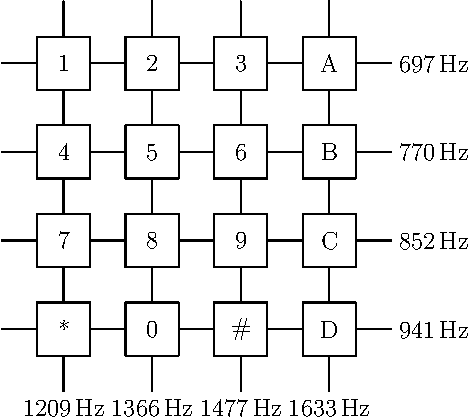
\includegraphics[height=.4\textheight]{figs/dtmf.pdf}
        \end{figure}
    \end{minipage}
\end{frame}

\begin{frame}[fragile]{\LaTeX{} 常用命令}
    \begin{exampleblock}{命令}
        \centering
        \footnotesize
        \begin{tabular}{llll}
            \cmd{chapter} & \cmd{section} & \cmd{subsection} & \cmd{paragraph} \\
            章 & 节 & 小节 & 带题头段落 \\\hline
            \cmd{centering} & \cmd{emph} & \cmd{verb} & \cmd{url} \\
            居中对齐 & 强调 & 原样输出 & 超链接 \\\hline
            \cmd{footnote} & \cmd{item} & \cmd{caption} & \cmd{includegraphics} \\
            脚注 & 列表条目 & 标题 & 插入图片 \\\hline
            \cmd{label} & \cmd{cite} & \cmd{ref} \\
            标号 & 引用参考文献 & 引用图表公式等\\\hline
        \end{tabular}
    \end{exampleblock}
    \begin{exampleblock}{环境}
        \centering
        \footnotesize
        \begin{tabular}{lll}
            \env{table} & \env{figure} & \env{equation}\\
            表格 & 图片 & 公式 \\\hline
            \env{itemize} & \env{enumerate} & \env{description}\\
            无编号列表 & 编号列表 & 描述 \\\hline
        \end{tabular}
    \end{exampleblock}
\end{frame}

\begin{frame}[fragile]{\LaTeX{} 环境命令举例}
    \begin{minipage}{0.5\linewidth}
\begin{lstlisting}[language=TeX]
\begin{itemize}
  \item A \item B
  \item C
  \begin{itemize}
    \item C-1
  \end{itemize}
\end{itemize}
\end{lstlisting}
    \end{minipage}\hspace{1cm}
    \begin{minipage}{0.3\linewidth}
        \begin{itemize}
            \item A
            \item B
            \item C
            \begin{itemize}
                \item C-1
            \end{itemize}
        \end{itemize}
    \end{minipage}
    \medskip
    \pause
    \begin{minipage}{0.5\linewidth}
\begin{lstlisting}[language=TeX]
\begin{enumerate}
  \item 巨佬 \item 大佬
  \item 萌新
  \begin{itemize}
    \item[n+e] 瑟瑟发抖
  \end{itemize}
\end{enumerate}
\end{lstlisting}
    \end{minipage}\hspace{1cm}
    \begin{minipage}{0.3\linewidth}
        \begin{enumerate}
            \item 巨佬
            \item 大佬
            \item 萌新
            \begin{itemize}
                \item[n+e] 瑟瑟发抖
            \end{itemize}
        \end{enumerate}
    \end{minipage}
\end{frame}

\begin{frame}[fragile]{\LaTeX{} 数学公式}
    \begin{columns}
        \begin{column}{.55\textwidth}
\begin{lstlisting}[language=TeX]
$V = \frac{4}{3}\pi r^3$

\[
  V = \frac{4}{3}\pi r^3
\]

\begin{equation}
  \label{eq:vsphere}
  V = \frac{4}{3}\pi r^3
\end{equation}
\end{lstlisting}
        \end{column}
        \begin{column}{.4\textwidth}
            $V = \frac{4}{3}\pi r^3$
            \[
                V = \frac{4}{3}\pi r^3
            \]
            \begin{equation}
                \label{eq:vsphere}
                V = \frac{4}{3}\pi r^3
            \end{equation}
        \end{column}
    \end{columns}
    \begin{itemize}
        \item 更多内容请看 \href{https://zh.wikipedia.org/wiki/Help:数学公式}{\color{purple}{这里}}
    \end{itemize}
\end{frame}

\begin{frame}[fragile]
    \begin{columns}
        \column{.6\textwidth}
\begin{lstlisting}[language=TeX]
    \begin{table}[htbp]
      \caption{编号与含义}
      \label{tab:number}
      \centering
      \begin{tabular}{cl}
        \toprule
        编号 & 含义 \\
        \midrule
        1 & 4.0 \\
        2 & 3.7 \\
        \bottomrule
      \end{tabular}
    \end{table}
    公式~(\ref{eq:vsphere}) 的
    编号与含义请参见
    表~\ref{tab:number}。
\end{lstlisting}
        \column{.4\textwidth}
        \begin{table}[htpb]
            \centering
            \caption{编号与含义}
            \label{tab:number}
            \begin{tabular}{cl}\toprule
                编号 & 含义 \\\midrule
                1 & 4.0\\
                2 & 3.7\\\bottomrule
            \end{tabular}
        \end{table}
        \normalsize 公式~(\ref{eq:vsphere})的编号与含义请参见表~\ref{tab:number}。
    \end{columns}
\end{frame}

\begin{frame}{作图}
    \begin{itemize}
        \item 矢量图 eps, ps, pdf
        \begin{itemize}
            \item METAPOST, pstricks, pgf $\ldots$
            \item Xfig, Dia, Visio, Inkscape $\ldots$
            \item Matlab / Excel 等保存为 pdf
        \end{itemize}
        \item 标量图 png, jpg, tiff $\ldots$
        \begin{itemize}
            \item 提高清晰度,避免发虚
            \item 应尽量避免使用
        \end{itemize}
    \end{itemize}
    \begin{figure}[htpb]
        \centering
        
\includegraphics[width=0.2\linewidth]{figs/ustc_logo.pdf}
        \caption{这个校徽就是矢量图}
    \end{figure}
\end{frame}

\begin{frame}{参考文献}
    \begin{itemize}
        \item 参考Transformer\cite{vaswani2017attention}
    \end{itemize}
\end{frame}

\section{计划进度}
\begin{frame}
    \begin{itemize}
        \item 一月:完成文献调研
        \item 二月:复现并评测各种Beamer主题美观程度
        \item 三、四月:美化SUDA Beamer主题
        \item 五月:论文撰写
    \end{itemize}
\end{frame}
% \section{计划进度}
\begin{frame}
    \begin{itemize}
        \item 一月:完成文献调研
        \item 二月:复现并评测各种Beamer主题美观程度
        \item 三、四月:美化SUDA Beamer主题
        \item 五月:论文撰写
    \end{itemize}
\end{frame}
% \section{总结}

\begin{frame}
    \begin{center}
        {\Huge\calligra 总结性文字}
    \end{center}
\end{frame}

\begin{frame}[allowframebreaks]
\begin{itemize}
    \item 参考文献:
\end{itemize}
    \scriptsize
    \bibliography{ref}
\end{frame}

\begin{frame}
    \begin{center}
        {\Huge\calligra Thanks!}
    \end{center}
\end{frame}



\section{Background}

\begin{frame}{Uniqueness of Movie Dubbing Task}
 \textbf{Movie dubbing}: Convert scripts to speeches, aligning with clip in timing and emotion, while preserving reference audio's timbre.\cite{zhang2024speaker}
    \begin{columns}[c]
        \column{0.6\textwidth}
        \begin{itemize}
            \item \textbf{Traditional VC/TTS}: Rely on the input text for modeling.
            \item \textbf{Movie dubbing}: Align with clip in emotion, rate, lip movements; preserve vocal timbre.
            \item \textbf{Transformed to one-to-one mapping.}
        \end{itemize}
        \column{0.4\textwidth}
        \begin{figure}
            \centering
            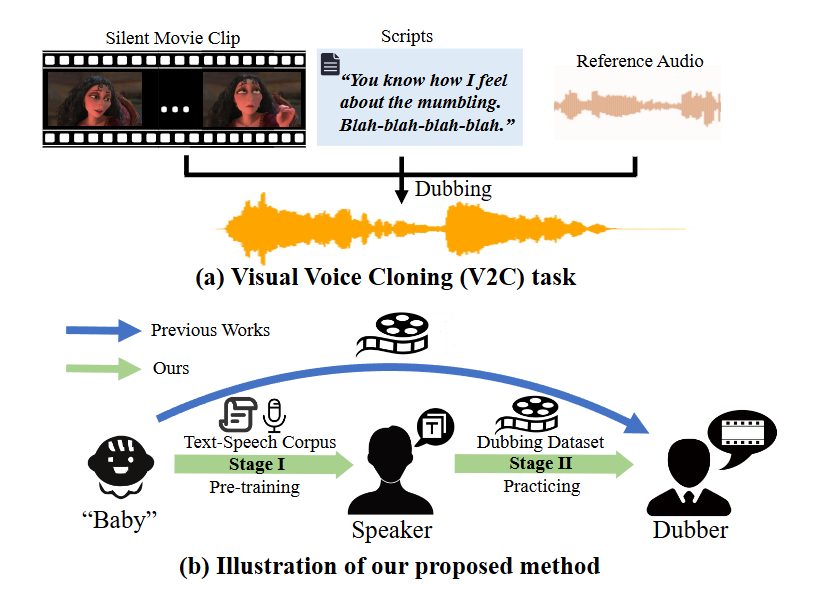
\includegraphics[width=\linewidth]{figs/difference.png}
            \caption{Movie dubbing vs. traditional VC/TTS}
            \label{fig:v2c_task}
        \end{figure}
    \end{columns}
\end{frame}


% \begin{frame}{Objectives of Movie Dubbing Task}
% \begin{columns}
%     \begin{column}{0.6\textwidth}
%         \begin{itemize}
%             \item Objectives of the movie dubbing task:
%             \begin{itemize}
%                 \item Preserve vocal timbre: Ensure a high match between the timbre of the dubbed speech and the reference audio.
%                 \item Synchronize emotion and speech rate: Align the emotional expression and speech rate of the dubbing with the performance of the characters in the movie clip.
%                 \item Align lip movements with speech: Match the duration of each phoneme in the dubbing with the lip movements of the characters.
%             \end{itemize}
%             \item The model needs to adapt to variations in emotion and speech rate while maintaining accurate pronunciation.
%         \end{itemize}
%     \end{column}
%     \begin{column}{0.4\textwidth}
%         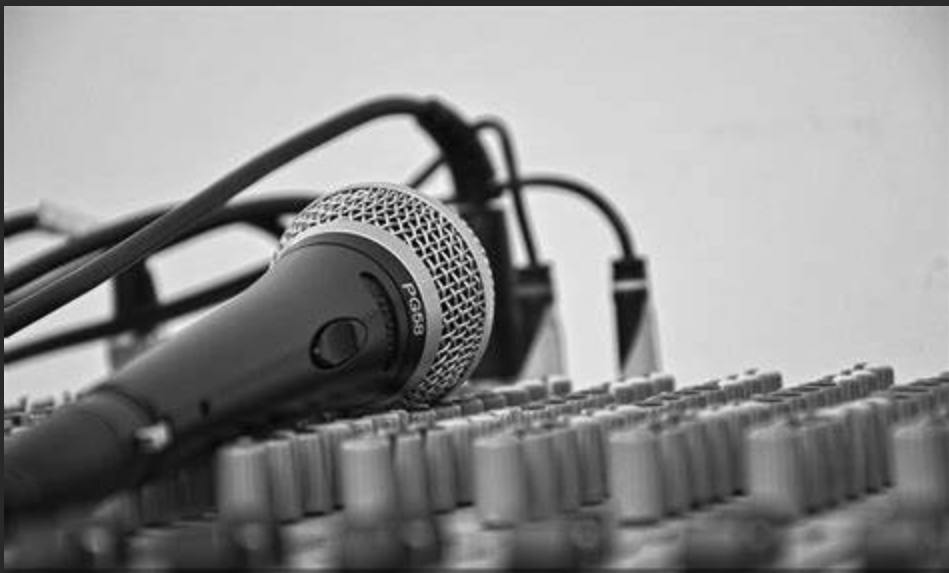
\includegraphics[width=\textwidth]{figs/配音.png} % Keep the original image path
%     \end{column}
% \end{columns}
% \end{frame}


\begin{frame}{Objectives of Movie Dubbing Task}
\textbf{The model needs to adapt to changes in emotion and speech speed to keep pronunciation accurate.}
\begin{columns}
    \begin{column}{0.6\textwidth}
        \begin{itemize}
                \item \textbf{Timbre}: Match dubbed speech to reference audio.
                \item \textbf{Emotion \& Rate}: Align with movie characters' performance.
                \item \textbf{Lip Sync}: Match phoneme duration to lip movements.
        \end{itemize}
    \end{column}
    \begin{column}{0.4\textwidth}
        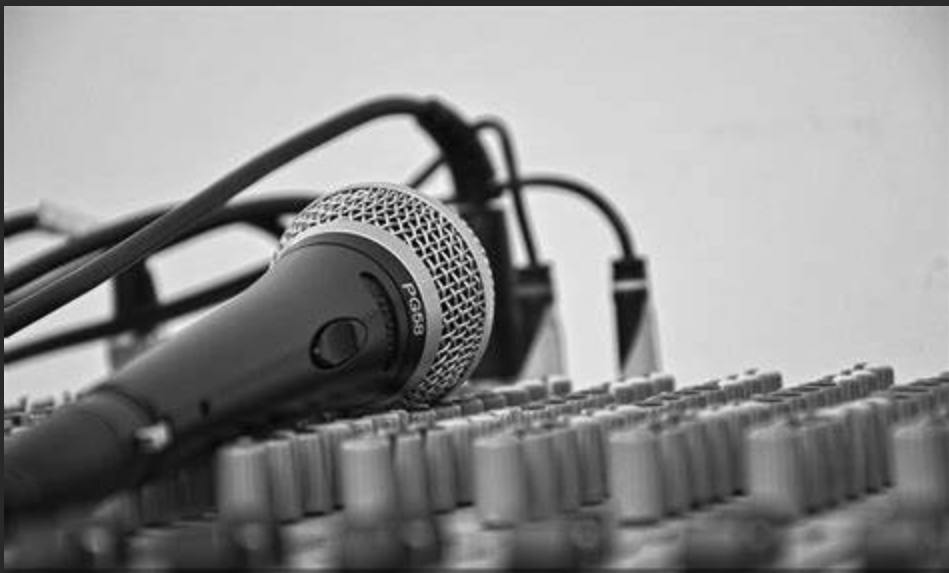
\includegraphics[width=\textwidth]{figs/配音.png}
    \end{column}
\end{columns}
\end{frame}



% \begin{frame}{Related Work}
% The Visual Voice Cloning (V2C) task \cite{chen2022v2c} requires the generated dubbing to align with the video content in terms of lip movements, emotions, and duration, which makes traditional speech synthesis methods inapplicable. To enhance the naturalness and consistency of dubbing, the authors draw on pre-training strategies and multi-modal alignment techniques.
% \begin{itemize}
% \item \textbf{Speech Synthesis:} Existing methods (e.g., the FastSpeech series) \cite{ren2020fastspeech} have made significant progress in speech synthesis, but they lack modeling of prosody and duration consistency with video content and thus cannot be directly applied to the V2C task.
% \item \textbf{Visual Voice Cloning:} The V2C task demands that the generated dubbing align with the video content in lip movements, emotions, and duration, significantly increasing the complexity of the task.
% \item \textbf{Pre-training in Text-to-Speech:} Pre-training strategies such as MP-BERT \cite{zhang2022mixed} and PLBERT \cite{li2023phoneme} enhance the naturalness of speech generation through phoneme-level modeling. These strategies are introduced into the V2C task in this paper to improve the quality of dubbing.
% \end{itemize}
% \end{frame}


\begin{frame}{Related Work}
The Visual Voice Cloning (V2C) task \cite{chen2022v2c} requires the generated dubbing to align with the video content in terms of lip movements, emotions, and duration, which makes traditional speech synthesis methods inapplicable. 
\begin{itemize}
    \item \textbf{Speech Synthesis:} FastSpeech\cite{ren2020fastspeech} series  excel in speech synthesis but lack video content alignment, making them unsuitable for V2C.
    \item \textbf{Visual Voice Cloning (V2C) :} Requires lip sync, emotion, and duration alignment with video, increasing task complexity.\cite{chen2022v2c}
    \item \textbf{Pre-training in TTS:} Strategies like MP-BERT \cite{zhang2022mixed} and PLBERT \cite{li2023phoneme} enhance speech naturalness via phoneme-level modeling, adopted in V2C to improve dubbing quality.
\end{itemize}
\end{frame}
\section{Paper Overview}
% \begin{frame}{Task Objective Description}
%     \frametitle{Task Objective Description}
%     The goal of the movie dubbing task is to generate dubbing that is consistent in timbre with the reference audio and aligned with the emotions and lip movements in the movie clip.
%     \begin{itemize}
%         \item The objective is to produce dubbing that matches the timbre of the reference audio while maintaining alignment with the emotions and lip movements in the movie clip.
%         \item This requires the model to accurately pronounce words while adapting to the emotional and pacing variations in the movie clip.
%     \end{itemize}
%     \vspace{1em}
%     \textbf{Movie Dubbing Task Formula:}
%     The model generates dubbing audio that matches the original video in terms of emotion, pacing, and duration based on the reference audio, script, and reference video.
%     \begin{equation}
%         \tilde{A}_{Dub} = Model(A_{Ref}, T_s, V_{Ref})
%     \end{equation}
% \end{frame}

\begin{frame}{Task Objective Description}
    \frametitle{Task Objective Description}
    \textbf{Task Goal:} Generate dubbing that matches reference audio's timbre and aligns with movie clip's emotions and lip movements.
    \begin{itemize}
        \item \textbf{Timbre Matching:} Align with reference audio.
        \item \textbf{Emotion \& Lip Sync:} Match movie clip's emotions and lip movements.
        \item \textbf{Accurate Pronunciation:} Adapt to emotional and pacing variations.
    \end{itemize}
    \vspace{1em}
    \textbf{Task Description with Formula for Movie Dubbing Task :}
    \begin{equation}
        \tilde{A}_{Dub} = Model(A_{Ref}, T_s, V_{Ref})
    \end{equation}
\end{frame}


% \begin{frame}{Overall Method Framework Overview}
%     \frametitle{Overall Method Framework Overview}
%     The framework consists of two main training stages: Multi-Task Speaker Pre-training (MTSP) and dubbing training, which includes Prosody Consistency Learning (PCL) and Duration Consistency Reasoning (DCR) modules.
%     \begin{figure}
%         \centering
%         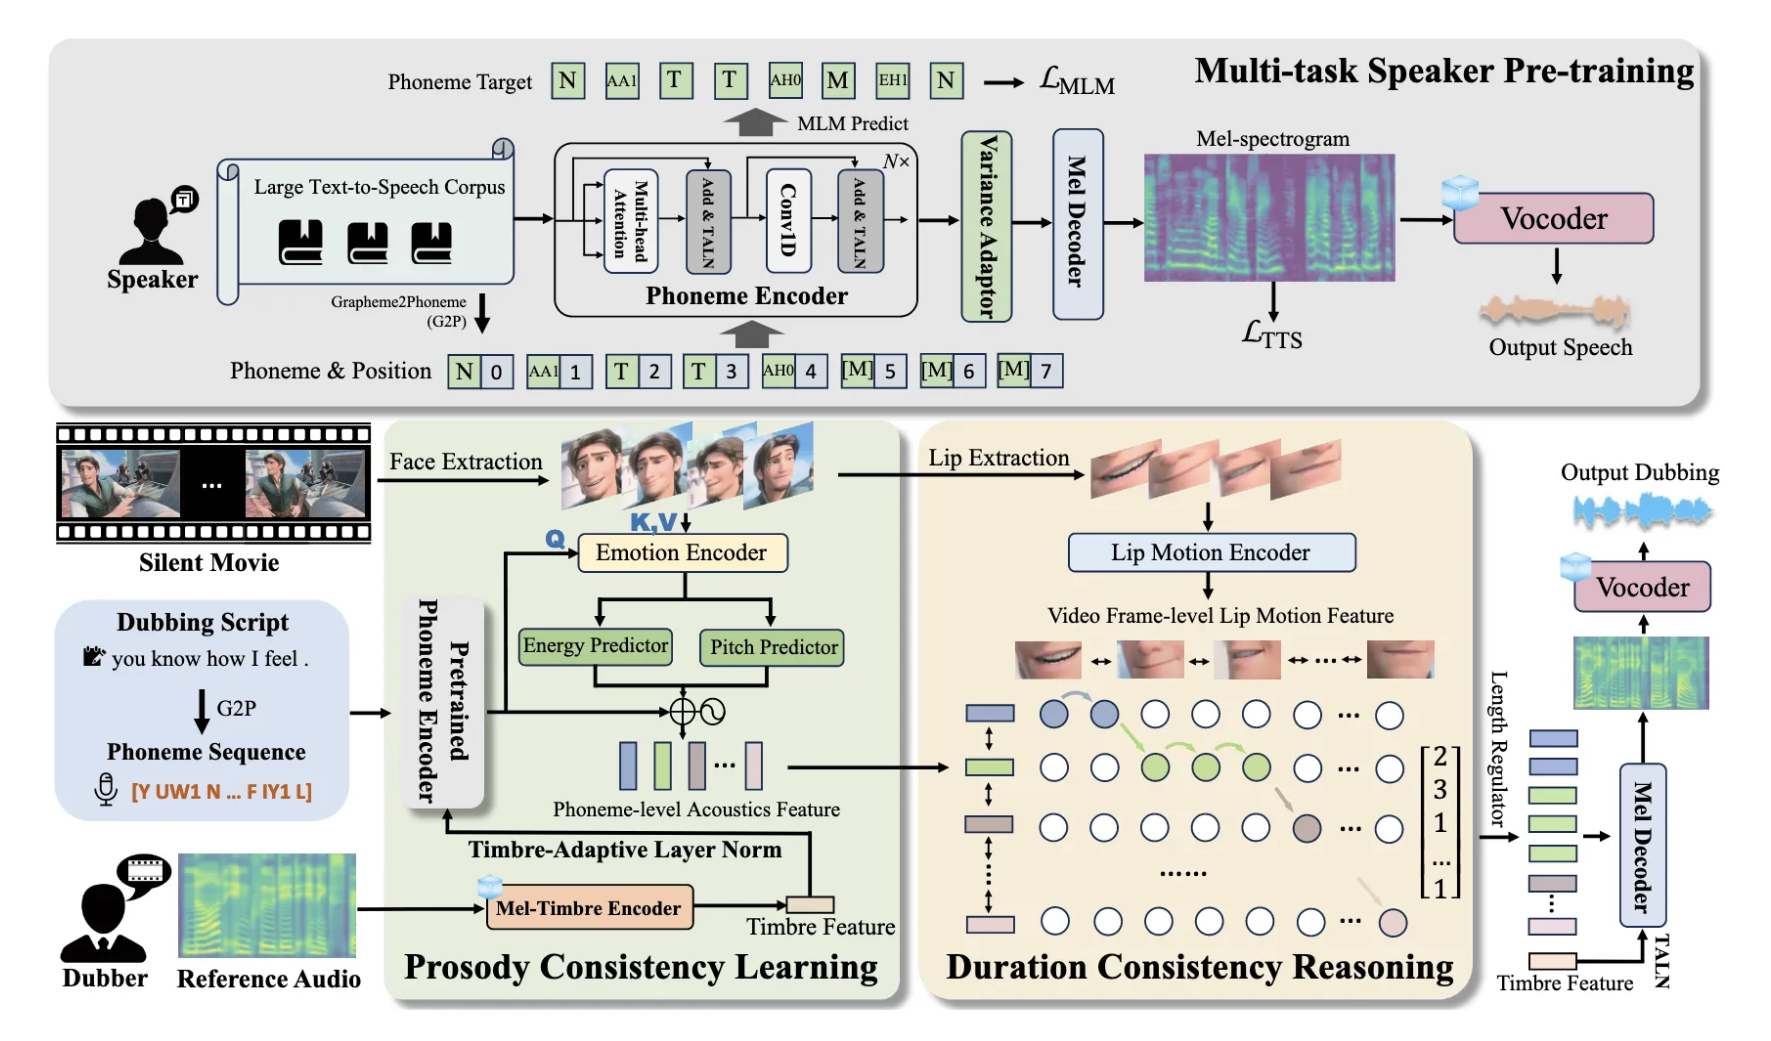
\includegraphics[width=0.6\textwidth]{figs/The main architecture.png} % Replace with your image path
%         \caption{The main architecture of the proposed two-stage dubbing method.}
%         \label{fig:method-framework}
%     \end{figure}
% \end{frame}

\begin{frame}{Overall Method Framework Overview}
    \frametitle{Overall Method Framework Overview}
    \textbf{Main Framework:}
    \begin{itemize}
        \item \textbf{MTSP:} Multi-Task Speaker Pre-training.Includes TTS task and MLM task
        \item \textbf{Dubbing Training:} Includes PCL (Prosody Consistency Learning) and DCR (Duration Consistency Reasoning).
    \end{itemize}
    \begin{figure}
        \centering
        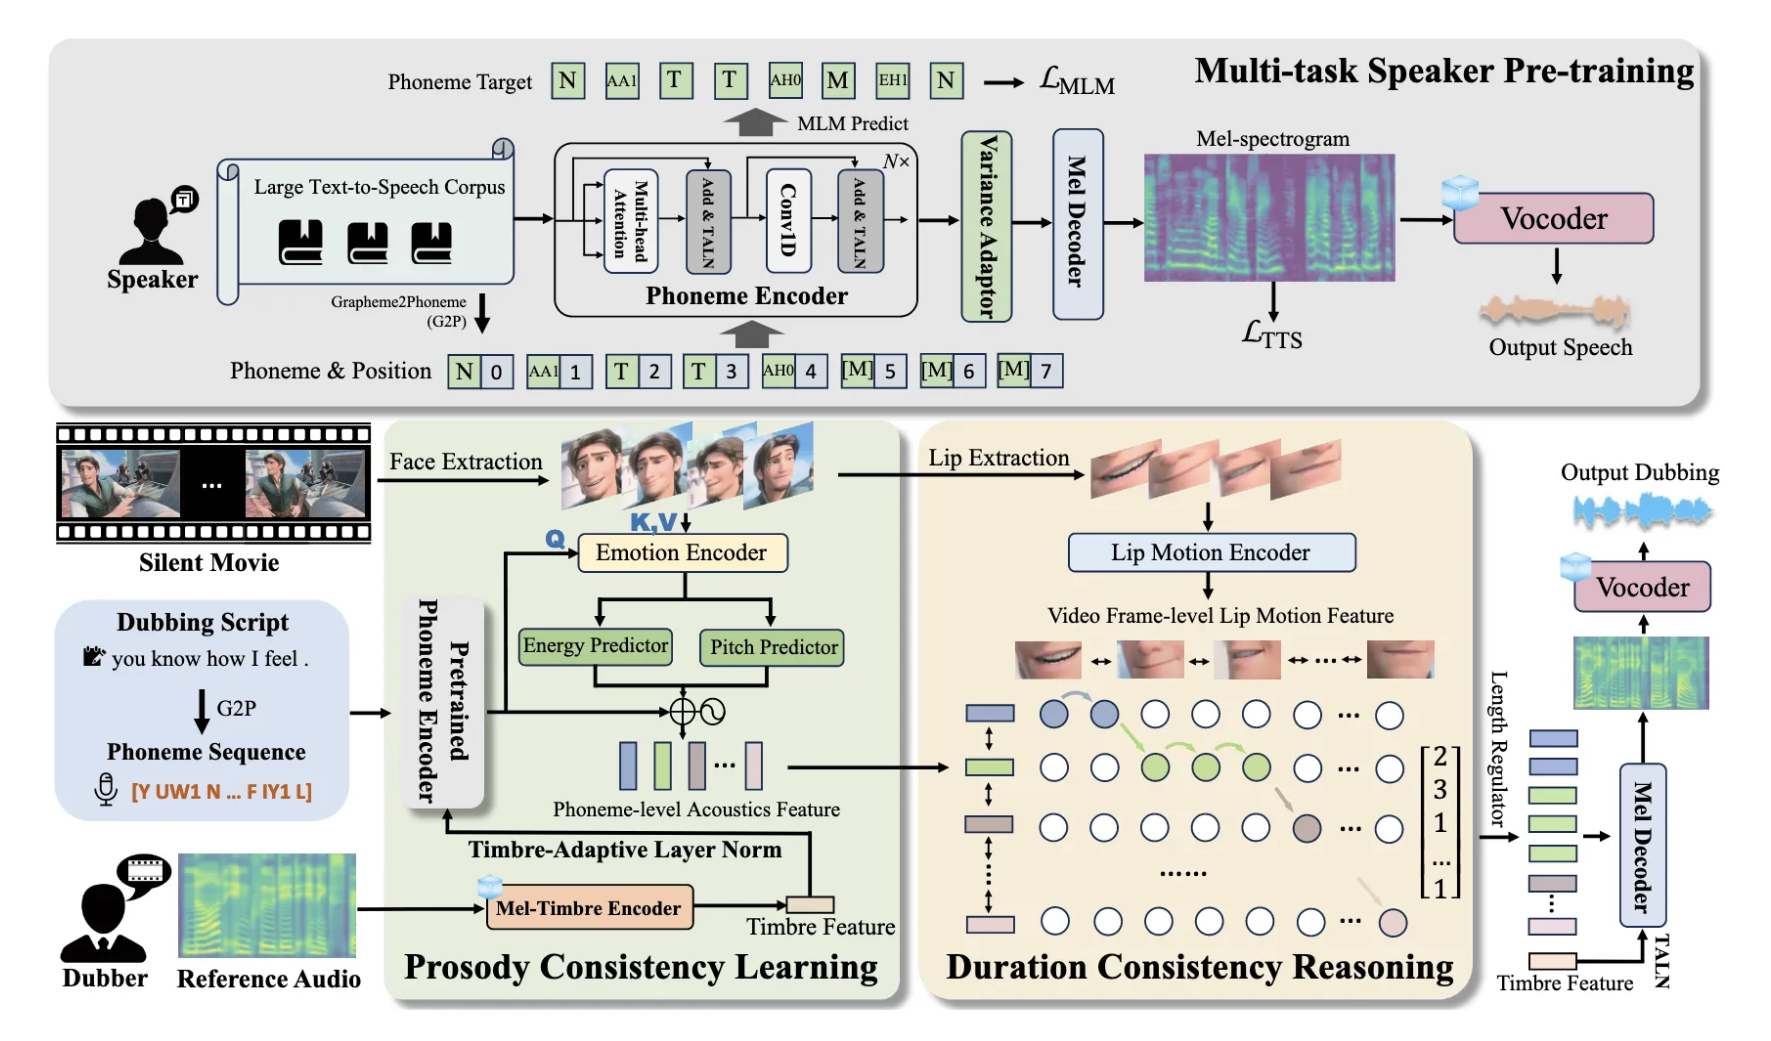
\includegraphics[width=0.45\textwidth]{figs/The main architecture.png}
        \caption{Main architecture of the two-stage dubbing method.}
        \label{fig:method-framework}
    \end{figure}
\end{frame}


% \begin{frame}{Detailed Description of the Overall Method Framework}
%     \frametitle{Detailed Description of the Overall Method Framework}
%     \begin{itemize}
%        \item \textbf{Stage 1: Multi-Task Speaker Pre-training (MTSP)}
%         \begin{itemize}
%             \item \textbf{Text-to-Speech (TTS) Task}
%             \begin{itemize}
%                 \item Objective: Learn accurate pronunciation representations from a large-scale text-to-speech corpus.
%                 \item Method: Use an architecture similar to FastSpeech2\cite{ren2020fastspeech} to predict the mel-spectrogram of the target speech.
%             \end{itemize}
%             \item \textbf{Masked Language Model (MLM) Prediction Task}
%             \begin{itemize}
%                 \item Objective: Learn contextual relationships between phonemes to better handle unseen text.
%                 \item Method: Convert text into phoneme sequences, randomly mask the sequences, and then predict the masked phoneme tokens.
%             \end{itemize}
%         \end{itemize}
%         \item \textbf{Stage 2: Dubbing Training}
%         \begin{itemize}
%             \item \textbf{Prosody Consistency Learning (PCL)}
%             \begin{itemize}
%                 \item Objective: Enhance audiovisual consistency.
%                 \item Method: Bridge the emotional states of characters in the movie clip with the phoneme-level prosody attributes of dubbing.
%             \end{itemize}
%             \item \textbf{Duration Consistency Reasoning (DCR)}
%             \begin{itemize}
%                 \item Objective: Ensure that the duration of the dubbing matches the video content.
%                 \item Method: Reason the phoneme-lip alignment and expand it to the mel length.
%             \end{itemize}
%         \end{itemize}
%     \end{itemize}
% \end{frame}

\begin{frame}{Detailed Description of the Overall Method Framework}
    \frametitle{Detailed Description of the Overall Method Framework}
    \begin{itemize}
        \item \textbf{Stage 1: Multi-Task Speaker Pre-training (MTSP)}
        \begin{itemize}
            \item \textbf{TTS Task:} Learn accurate pronunciation using FastSpeech2\cite{ren2020fastspeech} to predict target speech mel-spectrogram.
            \item \textbf{MLM Task:} Predict masked phonemes to capture phoneme context for unseen text.
        \end{itemize}
        \item \textbf{Stage 2: Dubbing Training}
        \begin{itemize}
            \item \textbf{PCL:} Enhance audiovisual consistency by aligning movie clip emotions with phoneme-level prosody.
            \item \textbf{DCR:} Ensure dubbing duration matches video content by reasoning phoneme-lip alignment.
        \end{itemize}
    \end{itemize}
\end{frame}
\section{MTSP}

% \begin{frame}{Multi-task Speaker Pre-training (MTSP)}
%     \frametitle{Multi-task Speaker Pre-training (MTSP)}
%     The goal of Multi-task Speaker Pre-training (MTSP) is to improve pronunciation clarity and naturalness through multi-task learning, thereby enhancing the quality of dubbing pronunciation.
%     \begin{itemize}
%         \item \textbf{TTS Task:} Learn accurate pronunciation representations from a text-to-speech corpus.
%         \item \textbf{MLM Prediction Task:} Learn contextual relationships between phonemes to better handle unseen text.
%     \end{itemize}
%     \textbf{Illustration of MTSP}
%     \begin{figure}[htpb]
%         \centering
%         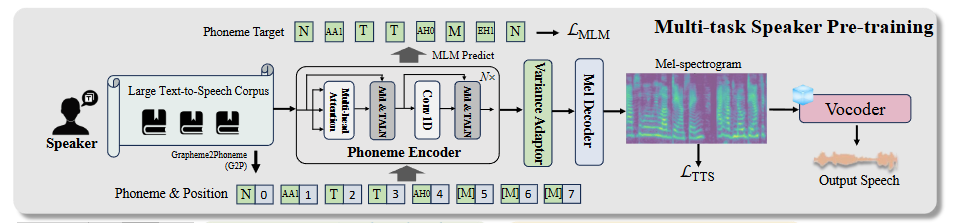
\includegraphics[width=0.8\textwidth]{figs/MSTP.png} % Replace with your image path
%         \caption{Illustration of Multi-task Speaker Pre-training}
%         \label{fig:mtsp}
%     \end{figure}
% \end{frame}
\begin{frame}{Multi-task Speaker Pre-training (MTSP)}
    \frametitle{Multi-task Speaker Pre-training (MTSP)}
    \textbf{Goal:} Improve pronunciation clarity and naturalness via multi-task learning.
    \begin{itemize}
        \item \textbf{TTS Task:} Learn accurate pronunciation from text-to-speech corpus.
        \item \textbf{MLM Task:} Capture phoneme context to handle unseen text.
    \end{itemize}
    \begin{figure}
        \centering
        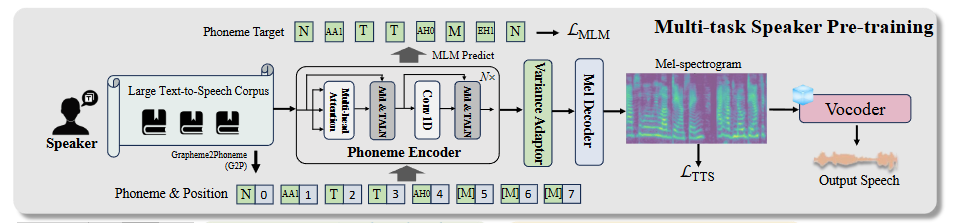
\includegraphics[width=0.8\textwidth]{figs/MSTP.png}
        \caption{Illustration of MTSP}
        \label{fig:mtsp}
    \end{figure}
\end{frame}

% \begin{frame}{TTS Task in MTSP}
%     \frametitle{TTS Task in MTSP}
%     \textbf{The TTS task enables the model to learn accurate pronunciation representations from a text-to-speech corpus} \\
%     Using an architecture similar to FastSpeech2, which includes a phoneme encoder, variance adaptor, and mel-decoder.
%     \begin{columns}[T] % Use top-aligned two columns
%         \column{0.6\textwidth} % Left column width is half of the text width
%         \begin{itemize}
%             \item Convert text to phoneme sequence: $T_p = \text{G2P}(T_o) $
%             \item The phoneme encoder extracts phoneme embeddings: $T_e = \text{PhonemeEncoder}(T_p) $
%             \item The variance adaptor models the prosody attributes of speech: $T_{\text{mel}} = \text{VarianceAdaptor}(E_{\text{ph}}, D_{\text{ph}}, P_{\text{ph}}, E_{\text{ph}})$
%         \end{itemize}
        
%         \column{0.4\textwidth} % Right column width is half of the text width
%         \begin{figure}[htpb]
%             \centering
%             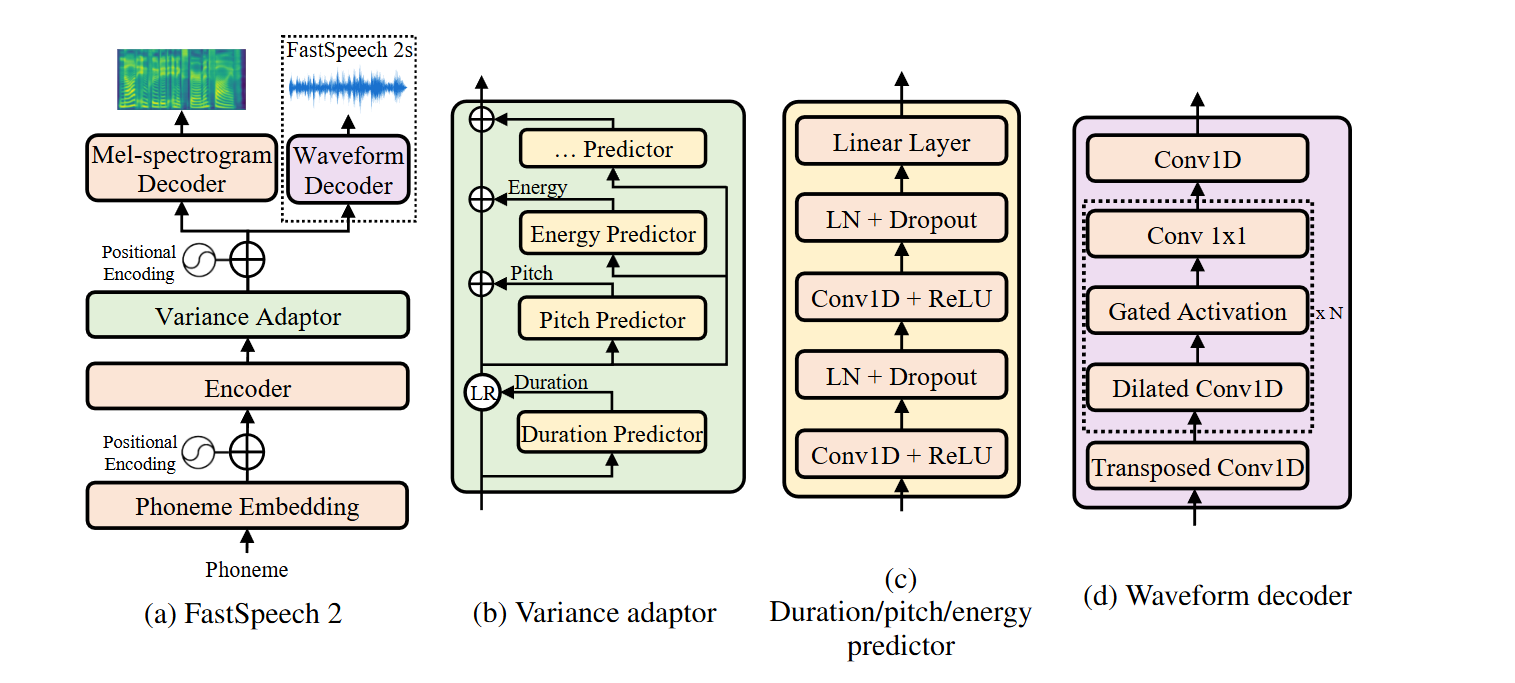
\includegraphics[width=\textwidth]{figs/fastSpeech架构图.png} % Replace with your image path
%             \caption{FastSpeech2 Architecture}
%             \label{fig:fastspeech2}
%         \end{figure}
%     \end{columns}
%     \vspace{1cm}
%     \textbf{Then predict the mel-spectrogram of the target speech and calculate the loss for the TTS task.}
% \end{frame}
\begin{frame}{TTS Task in MTSP}
    \frametitle{TTS Task in MTSP}
    \textbf{Objective:} Learn accurate pronunciation from text-to-speech corpus using FastSpeech2-like architecture.
    \begin{columns}[T] % Use top-aligned two columns
        \column{0.6\textwidth} % Left column width is 60% of the text width
        \begin{itemize}
            \item Convert text to phoneme sequence: $T_p = \text{G2P}(T_o)$
            \item Extract phoneme embeddings: $T_e = \text{PhonemeEncoder}(T_p)$
            \item Model prosody attributes: $T_{\text{mel}} = \text{VarianceAdaptor}(E_{\text{ph}}, D_{\text{ph}}, P_{\text{ph}}, E_{\text{ph}})$
        \end{itemize}
        
        \column{0.4\textwidth} % Right column width is 40% of the text width
        \begin{figure}[htpb]
            \centering
            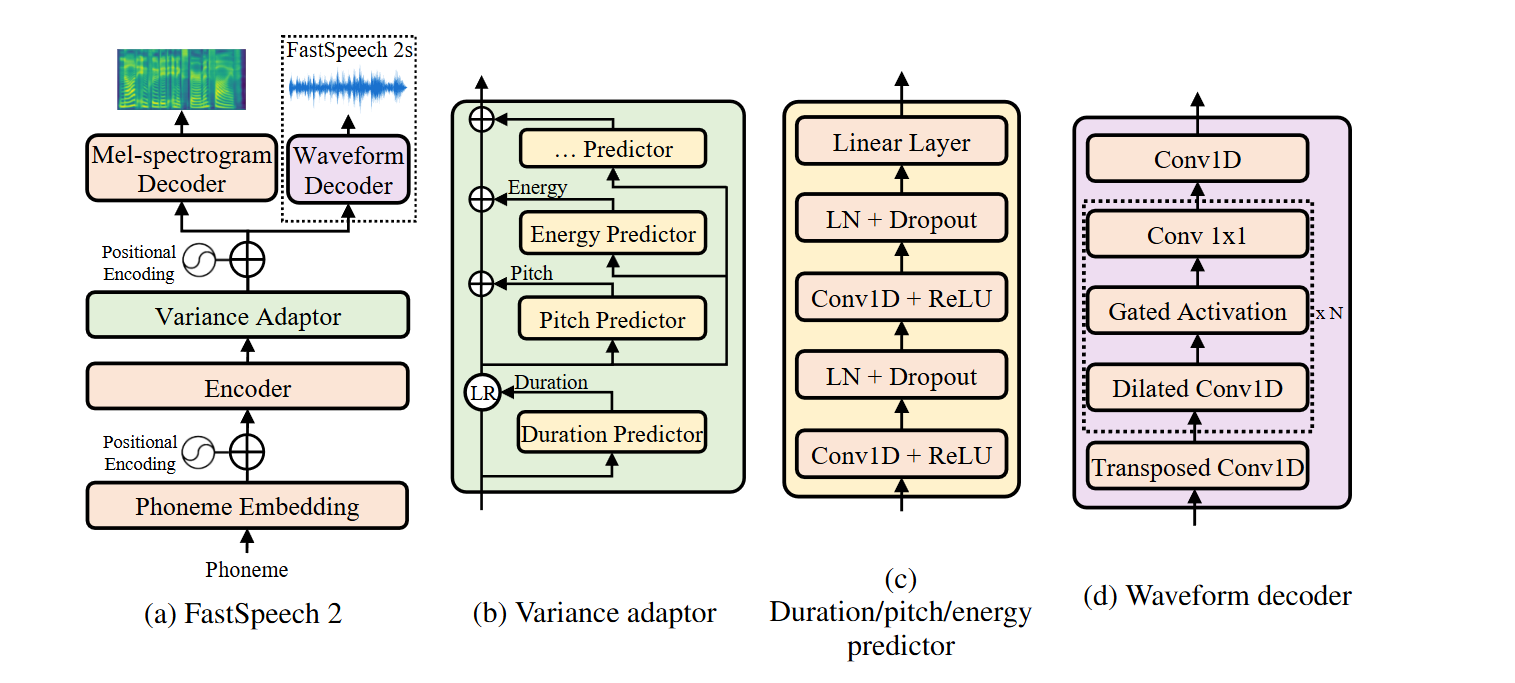
\includegraphics[width=\textwidth]{figs/fastSpeech架构图.png} % Replace with your image path
            \caption{FastSpeech2 Architecture}
            \label{fig:fastspeech2}
        \end{figure}
    \end{columns}
    \vspace{0.3cm}
    \textbf{Then predict the mel-spectrogram of the target speech and calculate the loss for the TTS task.}
\end{frame}

\begin{frame}{MLM Prediction Task in MTSP}
    \frametitle{MLM Prediction Task in MTSP}
    \textbf{The MLM prediction task helps the model learn contextual relationships between phonemes.}
    \begin{itemize}
        \item \textbf{Input:} Randomly masked phoneme sequence.
        \item \textbf{Processing:} Input to the phoneme encoder to predict the masked phonemes.
        \item \textbf{Output:} Predict the masked phonemes using linear projection and softmax function.
    \end{itemize}
    \textbf{MLM Prediction Task:}
    \begin{itemize}
        \item Predict the masked phonemes:
        \begin{equation}
            L_{\text{MLM}} = \text{CE}(\text{PhonemeEncoder}(T_{\text{masked}}), T_{\text{target}})
        \end{equation}
    \end{itemize}
\end{frame}


% \begin{frame}{Summary of MTSP}
%     \frametitle{Summary of MTSP}
%     \begin{itemize}
%         \item Multi-task Speaker Pre-training (MTSP) combines the Text-to-Speech (TTS) and Masked Language Model (MLM) tasks to improve the model's pronunciation quality and expressiveness.
%         \item The total loss function of MTSP integrates the losses of these two tasks, as shown in the formula:
%     \end{itemize}
%     \begin{equation}
%         \mathcal{L}_{MTSP} = \alpha_1 \cdot \mathcal{L}_{TTS} + \alpha_2 \cdot \mathcal{L}_{MLM},
%     \end{equation}
%     where, $\alpha_1$ and $\alpha_2$ are predefined hyperparameters, used to adjust the weights of the TTS and MLM tasks in the total loss.
% \end{frame}

\begin{frame}{Summary of MTSP}
    \frametitle{Summary of MTSP}
    \begin{itemize}
        \item \textbf{MTSP} combines \textbf{TTS} and \textbf{MLM} tasks to enhance pronunciation quality and expressiveness.
        \item Total loss function integrates losses of both tasks:
    \end{itemize}
    \begin{equation}
        \mathcal{L}_{MTSP} = \alpha_1 \cdot \mathcal{L}_{TTS} + \alpha_2 \cdot \mathcal{L}_{MLM},
    \end{equation}
    where $\alpha_1$ and $\alpha_2$ are hyperparameters adjusting task weights.
\end{frame}
\section{PCL}

% \begin{frame}
%     \frametitle{Overview of Prosody Consistency Learning (PCL)}
%     The Prosody Consistency Learning (PCL) module aims to enhance the audiovisual consistency of dubbing.
%     \begin{itemize}
%         \item \textbf{Method:} Model phoneme-level prosody attributes using emotional facial expression information. It is mainly divided into the following two parts:
%         \begin{columns}[T] % Use top-aligned two columns
%             \column{0.55\textwidth} % Left column width is half of the text width
%             \begin{itemize}
%                 \item \textbf{Alignment of Emotion and Prosody Attributes:} Align the emotional state of the character with the phoneme-level prosody attributes of dubbing through emotion feature extraction and cross-modal attention mechanism.
%                 \item \textbf{Timbre Consistency:} Ensure that the generated dubbing maintains timbre consistency with the reference audio through timbre feature extraction and Timbre-Adaptive Layer Normalization (TALN).
%             \end{itemize}
%             \column{0.45\textwidth} % Right column width is half of the text width
%             \begin{figure}[htpb]
%                 \centering
%                 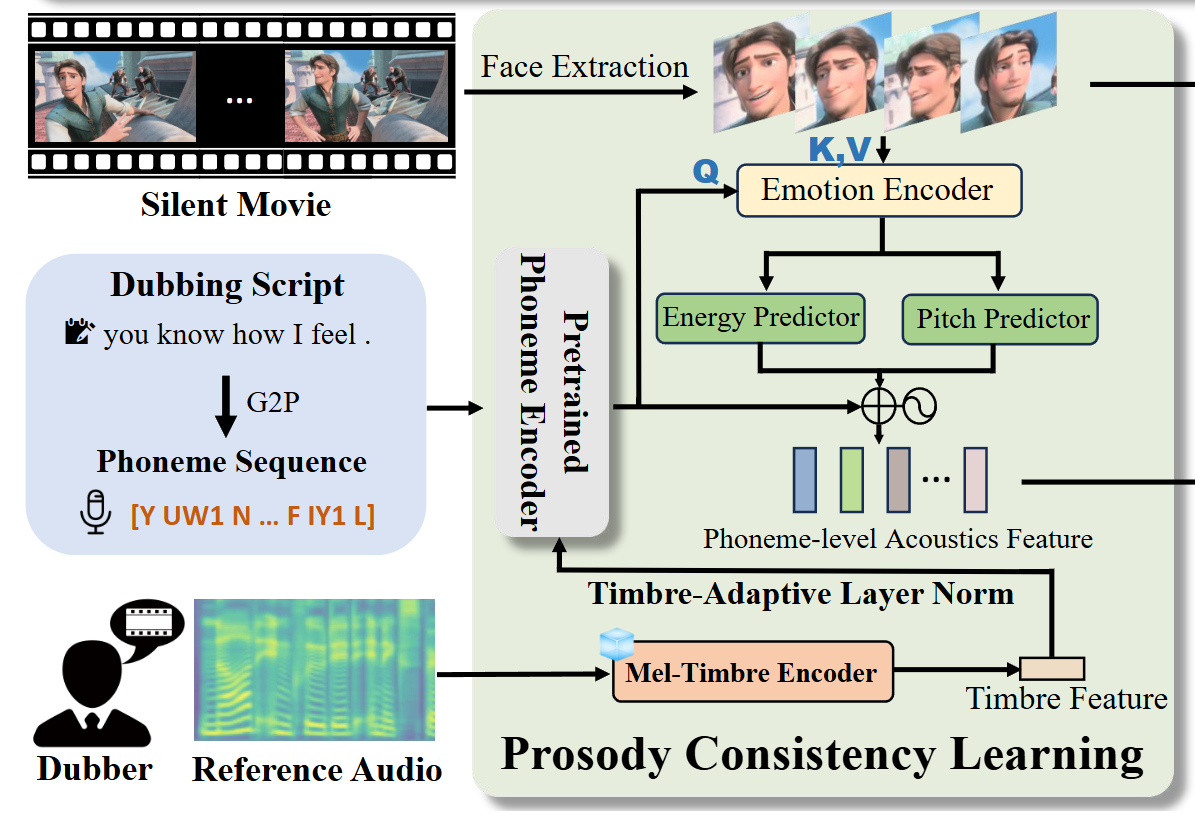
\includegraphics[width=\linewidth]{figs/PCL.png} % Replace with your image path
%                 \caption{Illustration of the PCL module}
%                 \label{fig:pcl-diagram}
%             \end{figure}
%         \end{columns}
%     \end{itemize}
% \end{frame}
\begin{frame}
    \frametitle{Overview of Prosody Consistency Learning (PCL)}
    \textbf{Objective:} Enhance audiovisual consistency of dubbing.
    \begin{itemize}
        \item \textbf{Method:} Model phoneme-level prosody using emotional facial expressions. Key components:
        \begin{columns}[c] % Use top-aligned two columns
            \column{0.55\textwidth} % Left column width
            \begin{itemize}
                \item \textbf{Emotion-Prosody Alignment:} Align character emotions with phoneme-level prosody via cross-modal attention.
                \item \textbf{Timbre Consistency:} Maintain reference audio's timbre using TALN.
            \end{itemize}
            \column{0.45\textwidth} % Right column width
            \begin{figure}
                \centering
                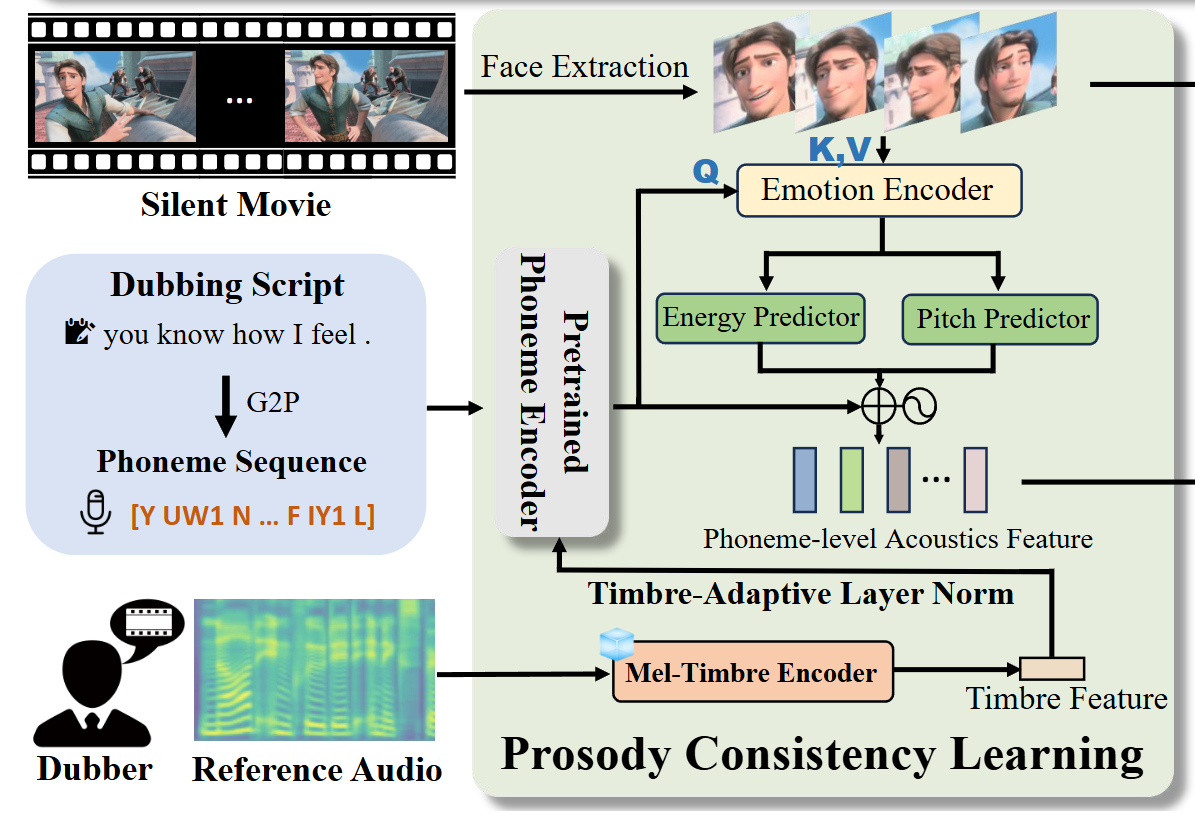
\includegraphics[width=\linewidth]{figs/PCL.png}
                \caption{PCL module illustration}
                \label{fig:pcl-diagram}
            \end{figure}
        \end{columns}
    \end{itemize}
\end{frame}


% \begin{frame}{Prosody Consistency Learning (PCL)}
% \framesubtitle{(1) Alignment of Emotion and Prosody Attributes}
% \begin{itemize}
%     \item \textbf{Objective:} Align the emotional state of the character in the movie clip with the phoneme-level prosody attributes (pitch and energy) of the dubbing while ensuring that the timbre of the dubbing remains consistent with the reference audio.
%     \item \textbf{Steps Introduction:}
%     \begin{enumerate}
%         \item \textbf{Emotion Feature Extraction:} Extract and encode emotional features from facial regions.
%         \item \textbf{Cross-modal Attention Mechanism:} Use attention mechanisms to align emotional features with phoneme prosody attributes.
%         \item \textbf{Prediction of Phoneme Pitch and Energy:} Predict the pitch and energy of phonemes and embed them into the phoneme sequence.
%     \end{enumerate}
%     \item \textbf{Step 1: Emotion Feature Extraction}
%     \begin{itemize}
%         \item Extract the facial region of each frame in the movie clip using S3FD face detection:
%         \begin{equation}
%             V_{\text{face}} = S^3FD(V_{\text{Ref}}) \in \mathbb{R}^{L_v \times H_{\text{face}} \times W_{\text{face}} \times C}
%         \end{equation}
%         \item Encode the facial region into emotional features using the EmoFAN network:
%         \begin{equation}
%             V_{\text{emo}} = \text{EmoFAN}(V_{\text{face}}) \in \mathbb{R}^{L_v \times d_m}
%         \end{equation}
%     \end{itemize}
% \end{itemize}
% \end{frame}
\begin{frame}{Prosody Consistency Learning (PCL)}
\framesubtitle{(1) Alignment of Emotion and Prosody Attributes}
\begin{itemize}
    \item \textbf{Objective:} Align character emotions with phoneme-level prosody (pitch and energy) while maintaining reference audio's timbre.
    \item \textbf{Steps:}
    \begin{enumerate}
        \item \textbf{Extract Emotion Features:} Detect faces with S3FD, encode emotions with EmoFAN.
        \item \textbf{Cross-modal Attention:} Align emotion features with phoneme prosody.
        \item \textbf{Predict Phoneme Attributes:} Embed predicted pitch and energy into phoneme sequence.
    \end{enumerate}
    \item \textbf{Step 1: Emotion Feature Extraction}
    \begin{itemize}
        \item Detect facial regions using S3FD:
        \begin{equation}
            V_{\text{face}} = S^3FD(V_{\text{Ref}}) \in \mathbb{R}^{L_v \times H_{\text{face}} \times W_{\text{face}} \times C}
        \end{equation}
        \item Encode emotions using EmoFAN:
        \begin{equation}
            V_{\text{emo}} = \text{EmoFAN}(V_{\text{face}}) \in \mathbb{R}^{L_v \times d_m}
        \end{equation}
    \end{itemize}
\end{itemize}
\end{frame}

\begin{frame}{Prosody Consistency Learning (PCL)}
\framesubtitle{(1) Alignment of Emotion and Prosody Attributes}

\begin{itemize}
    \item \textbf{Step 2: Cross-modal Attention Mechanism}
    \begin{itemize}
    \item Use multi-head cross-modal attention to align the emotional features of the character with the prosody attributes of each phoneme:
        \begin{equation}
            \xi_{\text{pho,pitch}}^k = \text{softmax}\left(\frac{Q^{\top} K_p}{\sqrt{d_m}}\right) V_p \in \mathbb{R}^{L_p \times \frac{d_m}{n_{\text{head}}}}
        \end{equation}
        \begin{equation}
            \xi_{\text{pho,energy}}^k = \text{softmax}\left(\frac{Q^{\top} K_e}{\sqrt{d_m}}\right) V_e \in \mathbb{R}^{L_p \times \frac{d_m}{n_{\text{head}}}}
        \end{equation}
        \item Where:
        \begin{equation}
            Q = W_j^Q T_e^{\top}, \quad K_p = W_j^{K_p} V_{\text{emo}}^{\top}, \quad V_p = W_j^{V_p} V_{\text{emo}}^{\top}
        \end{equation}
        \begin{equation}
            K_e = W_j^{K_e} V_e^{\top}, \quad V_e = W_j^{V_e} V_{\text{emo}}^{\top}
        \end{equation}
    \end{itemize}
\end{itemize}
\end{frame}


\begin{frame}{Prosody Consistency Learning (PCL)}
\framesubtitle{(1) Alignment of Emotion and Prosody Attributes}

\begin{itemize}
    \item  \textbf{Step 3: Prediction of Phoneme Pitch and Energy}
    \begin{itemize}
        \item Use pitch and energy predictors to predict the pitch and energy of each phoneme, convert them into pitch and energy embeddings, and then add them to the phoneme sequence:
        \begin{equation}
            \tilde{P}_{\text{pho}}, \tilde{E}_{\text{pho}} = \text{Predictor}(\xi_{\text{pho,pitch}}, \xi_{\text{pho,energy}}) \in \mathbb{N}^{L_p}
        \end{equation}
        \item Add pitch and energy embeddings to the phoneme sequence:
        \begin{equation}
            T_a = T_e + \text{PitchEmb}(\tilde{P}_{\text{pho}}) + \text{EnergyEmb}(\tilde{E}_{\text{pho}})
        \end{equation}
    \end{itemize}
\end{itemize}
\end{frame}


% \begin{frame}{Prosody Consistency Learning (PCL)}
% \framesubtitle{(2) Timbre Consistency}
% \begin{itemize}
%     \item \textbf{Objective:} Accurately replicate the timbre of the reference audio.
%     \item \textbf{Method:} Use Timbre-Adaptive Layer Normalization (TALN) to integrate the timbre feature into phoneme encoding and mel-spectrogram generation by predicting the gain and bias of the input vector sequence.
%     \item \textbf{Formula:}
%     \begin{equation}
%         \text{TALN}(x, E_{\text{timbre}}) = \text{gain}(E_{\text{timbre}}) \frac{x - \mu}{\sigma} + \text{bias}(E_{\text{timbre}})
%     \end{equation}
%     \item \textbf{Parameter Explanation:}
%     \begin{itemize}
%         \item \( x \) and \( E_{\text{timbre}} \) are the input sequence and timbre feature, respectively.
%         \item \( \mu \), \( \sigma \) are the mean and variance of \( x \), respectively.
%         \item \( \text{gain}(\cdot) \) and \( \text{bias}(\cdot) \) are the prediction functions for gain and bias, respectively.
%     \end{itemize}
%     \item \textbf{Application:} The proposed TALN is applied to each FFT block of the phoneme encoder and mel-decoder to integrate the vocal timbre feature.
% \end{itemize}
% \end{frame}

\begin{frame}{Prosody Consistency Learning (PCL)}
\framesubtitle{(2) Timbre Consistency}
\begin{itemize}
    \item \textbf{Objective:} Replicate reference audio's timbre accurately.
    \item \textbf{Method:} Use TALN to integrate timbre features into phoneme encoding and mel-spectrogram generation.
    \item \textbf{Formula:}
    \begin{equation}
        \text{TALN}(x, E_{\text{timbre}}) = \text{gain}(E_{\text{timbre}}) \frac{x - \mu}{\sigma} + \text{bias}(E_{\text{timbre}})
    \end{equation}
    \item \textbf{Parameters:}
    \begin{itemize}
        \item \( x \): Input sequence.
        \item \( E_{\text{timbre}} \): Timbre feature.
        \item \( \mu \), \( \sigma \): Mean and variance of \( x \).
        \item \( \text{gain}(\cdot) \), \( \text{bias}(\cdot) \): Predicted gain and bias.
    \end{itemize}
    \item \textbf{Application:} Apply TALN to each FFT block of phoneme encoder and mel-decoder.
\end{itemize}
\end{frame}
\section{DCR}

% \begin{frame}
%     \frametitle{Overview of Duration Consistency Alignment}
%     The Duration Consistency Alignment module aims to enhance the temporal consistency of the dubbed audio.
%     \begin{itemize}
%         \item \textbf{Method:} Achieve optimal alignment of phoneme-level durations through lip motion feature extraction and dynamic programming algorithms. It is mainly divided into three parts:
%     \end{itemize}
%     \begin{columns}[T] % Use top-aligned two columns
%         \column{0.55\textwidth} % Left column width is 55% of the text width
%         \textbf{Module Composition:}
%         \begin{itemize}
%             \item \textbf{Lip Motion-Phoneme Alignment:} Extract lip motion features and compute the similarity matrix with phoneme features.
%             \item \textbf{Phoneme Duration Expansion:} Use dynamic programming to find the optimal alignment and expand phoneme durations.
%             \item \textbf{Mel-Spectrogram Duration Expansion:} Expand the length of the mel-spectrogram based on audio duration.
%         \end{itemize}
%         \column{0.3\textwidth} % Right column width is 45% of the text width
%         \begin{figure}[htpb]
%             \centering
%             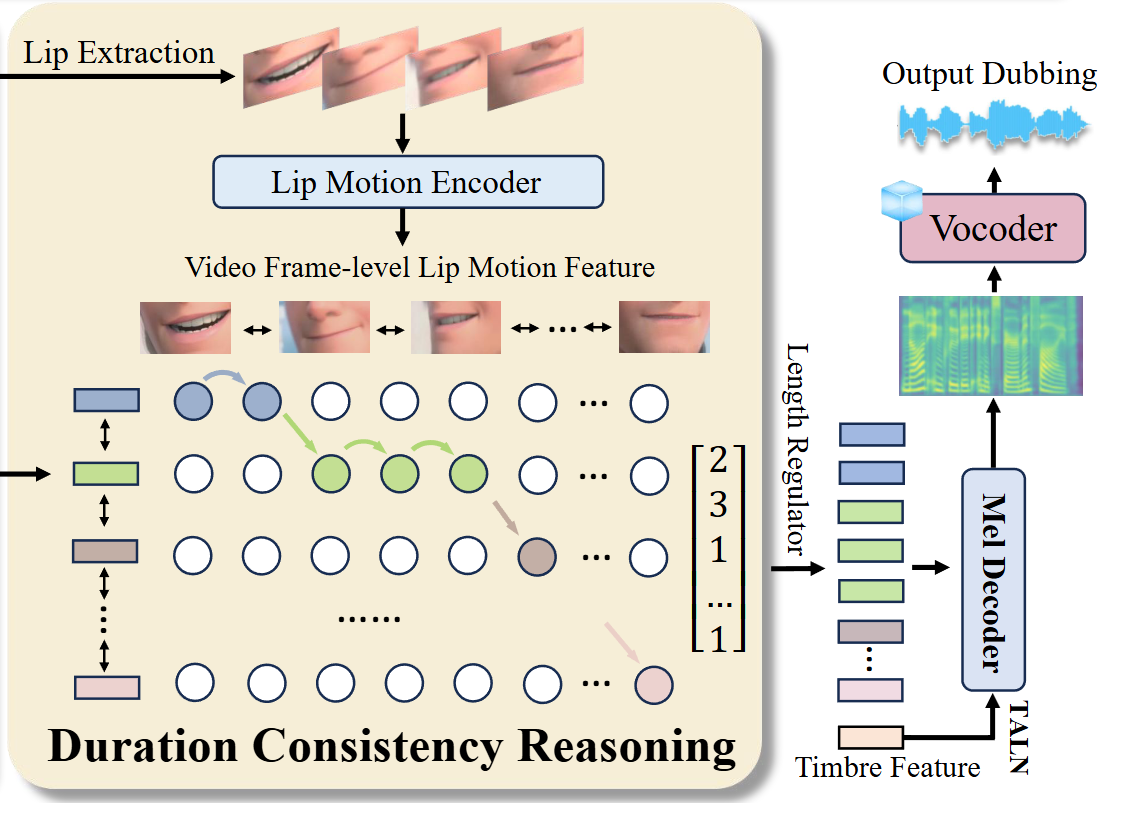
\includegraphics[width=\linewidth]{figs/DCR.png} % Replace with your image path
%             \caption{Illustration of the DCR module}
%             \label{fig:dcr-diagram}
%         \end{figure}
%     \end{columns}
% \end{frame}
\begin{frame}
    \frametitle{Overview of Duration Consistency Alignment}
    \textbf{Objective:} Enhance temporal consistency of dubbed audio.
    \begin{columns}[T] % Use top-aligned two columns
        \column{0.55\textwidth} % Left column width is 55% of the text width
        \textbf{Module Composition:}
        \begin{itemize}
            \item \textbf{Lip Motion-Phoneme Alignment:} Extract lip motion features and align with phoneme features.
            \item \textbf{Phoneme Duration Expansion:} Use dynamic programming to optimize phoneme durations.
            \item \textbf{Mel-Spectrogram Duration Expansion:} Adjust mel-spectrogram length based on audio duration.
        \end{itemize}
        \column{0.3\textwidth} % Right column width is 30% of the text width
        \begin{figure}
            \centering
            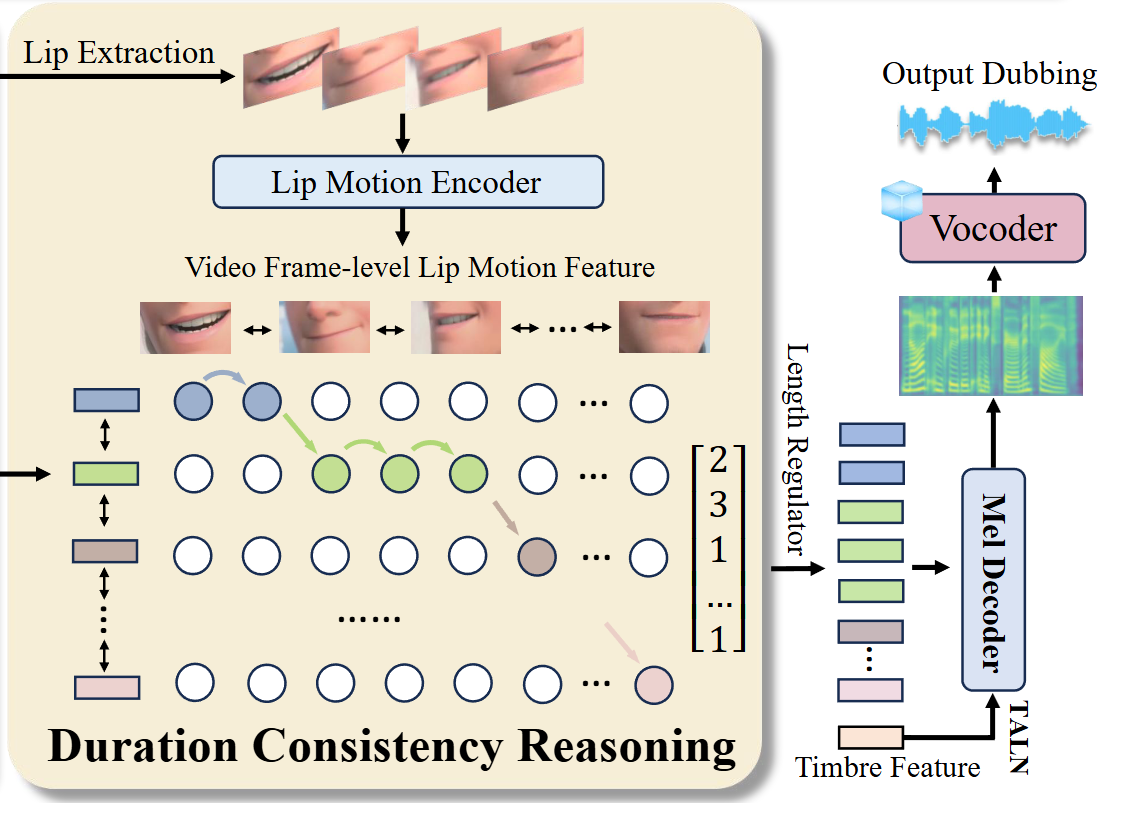
\includegraphics[width=\linewidth]{figs/DCR.png} % Replace with your image path
            \caption{DCR module illustration}
            \label{fig:dcr-diagram}
        \end{figure}
    \end{columns}
\end{frame}


\begin{frame}{Duration Consistency Alignment (DCR)}
\framesubtitle{(1) Lip Motion-Phoneme Alignment}
\begin{itemize}
    \item \textbf{Step 1: Lip Motion-Phoneme Alignment}
    \begin{itemize}
    \item \textbf{Objective:} Extract lip motion features from the reference video and align them with phoneme features.
    \item \textbf{Steps:}
    \begin{enumerate}
        \item Extract the lip motion region from the video:
        \begin{equation}
            V_{\text{lip}} \in \mathbb{R}^{L_v \times H_{\text{lip}} \times W_{\text{lip}} \times C}
        \end{equation}
        \item Obtain the lip motion representation using a lip motion encoder:
        \begin{equation}
            E_{\text{lip}} \in \mathbb{R}^{L_v \times d_{\text{model}}}
        \end{equation}
    \end{enumerate}
\end{itemize}
\end{itemize}

\end{frame}

\begin{frame}{Duration Consistency Alignment (DCR)}
\framesubtitle{(2) Phoneme Duration Expansion}
\begin{itemize}
    \item \textbf{Step 2: Phoneme Duration Expansion}
    \begin{itemize}
    \item \textbf{Objective:} Expand phoneme durations to match lip motion features.
    \item \textbf{Steps:}
    \begin{enumerate}
        \item \textbf{Similarity Matrix Calculation:} Compute the similarity matrix between phoneme-level acoustic features and lip motion features.
        \begin{equation}
            S_{\text{pho,lip}} = \text{Similarity}(T_a^i, E_{\text{lip}}^j)
        \end{equation}
        \item \textbf{Dynamic Programming Alignment:} Use dynamic programming to find the optimal alignment.
        \begin{equation}
            A_{i,j} = 
            \begin{cases} 
                \text{None}, & \text{if } i > j \text{ or } j - i < L_p - L_{\text{p}} \\
                \max(A_{i-1,j}, A_{i-1,j-1}) + s_{i,j}, & \text{otherwise}
            \end{cases}
        \end{equation}
    \end{enumerate}
\end{itemize}
\end{itemize}
\end{frame}


\begin{frame}{Duration Consistency Alignment (DCR)}
\framesubtitle{(3) Mel-Spectrogram Duration Expansion}
\begin{itemize}
    \item \textbf{Step 3: Mel-Spectrogram Duration Expansion}
    \begin{itemize}
    \item \textbf{Objective:} Expand the length of the mel-spectrogram to match the audio duration.
    \item \textbf{Steps:}
    \begin{enumerate}
        \item \textbf{Fixed Ratio Relationship:} Expand the length of the mel-spectrogram based on audio duration.
        \begin{equation}
            n = \frac{L_{\text{mel}}}{L_0} = \frac{sr/hs}{FPS} \in \mathbb{N}^*
        \end{equation}
        \item \textbf{Mel-Spectrogram Generation:} Use a length regulator to generate the mel-spectrogram of the desired length:
        \begin{equation}
            \tilde{A}_{\text{Dub}} = \text{Vocoder}(\text{MelDecoder}(LR(T_a, A^* \times n), E_{\text{imbr}}))
        \end{equation}
    \end{enumerate}
\end{itemize}
\end{itemize}
\end{frame}
\section{Experiments}

\begin{frame}
\frametitle{Experimental Results: Comparison with SOTA}
\begin{itemize}
    \item Key metrics maintain high levels across multiple datasets
    \begin{columns}[T]
    \column{0.3\textwidth}
    \begin{figure}[H]
        \centering
        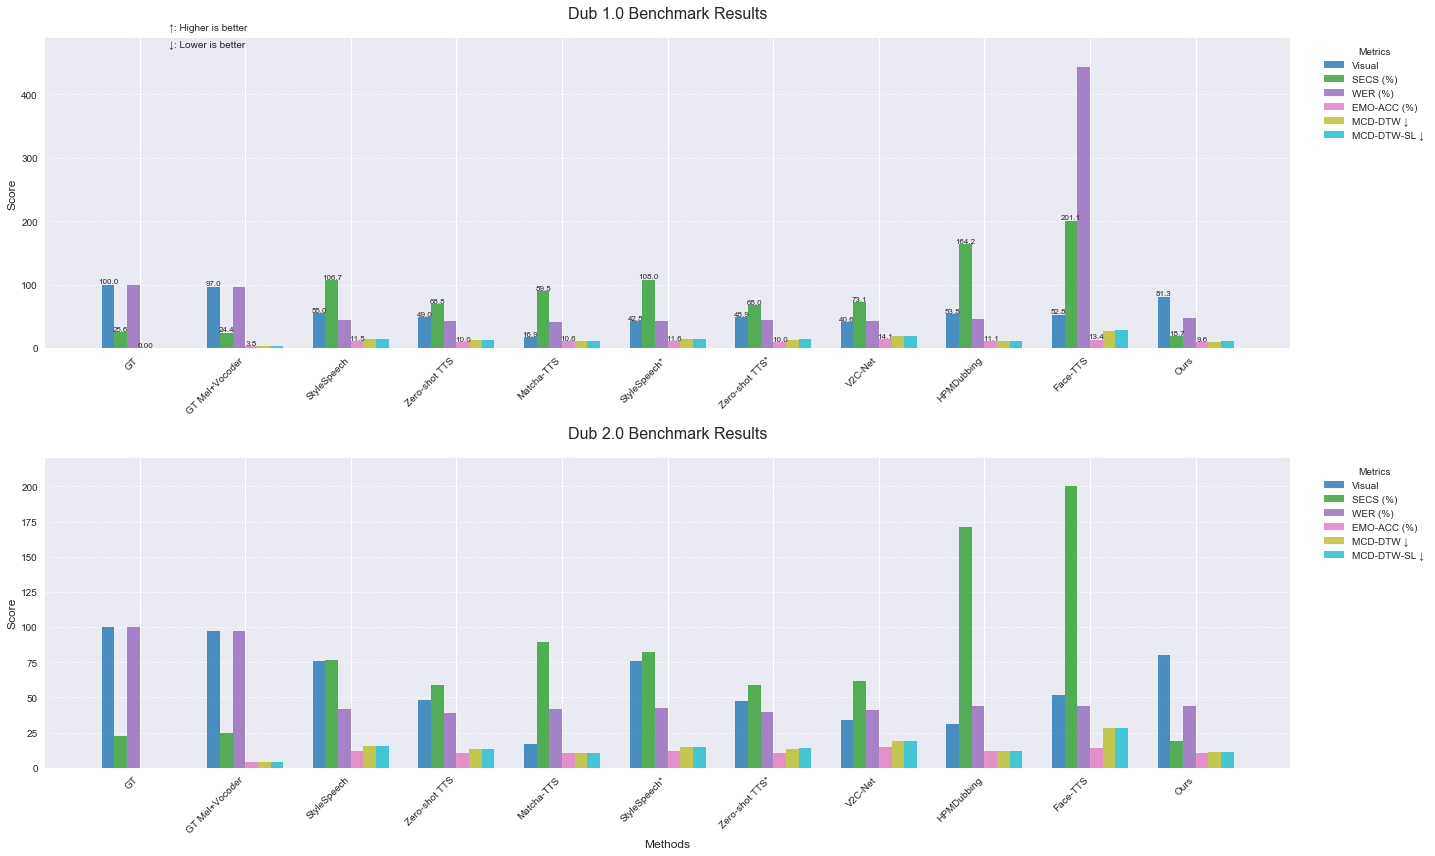
\includegraphics[width=\linewidth]{figs/1table.png} % Replace with the image path for V2C-Animation dataset results
        \caption{V2C-A Dataset Test Results}
        \label{fig:v2c-animation}
    \end{figure}

    \column{0.3\textwidth}
    \begin{figure}[H]
        \centering
        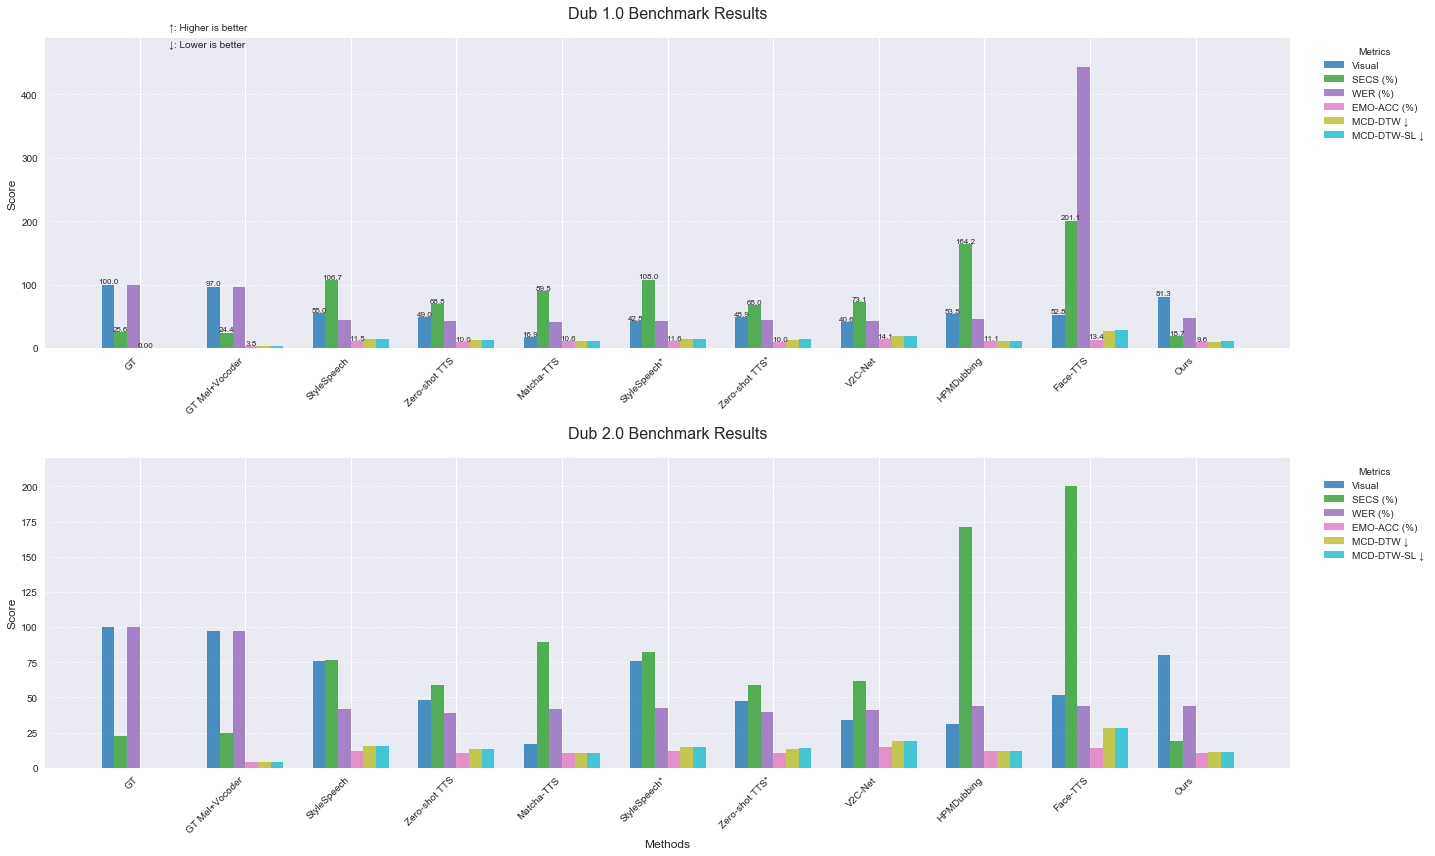
\includegraphics[width=\linewidth]{figs/1table.png} % Replace with the image path for GRID dataset results
        \caption{GRID Dataset Test Results}
        \label{fig:grid}
    \end{figure}
\end{columns}

\begin{columns}[T]
    \column{0.3\textwidth}
    \begin{figure}[H]
        \centering
        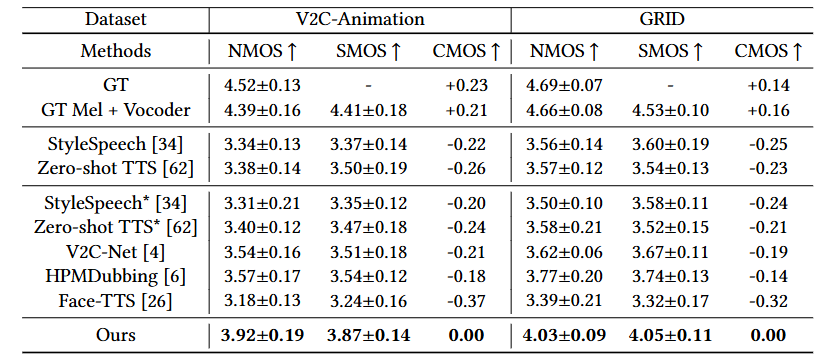
\includegraphics[width=\linewidth]{figs/table3.png} % Replace with the image path for zero-shot test results
        \caption{Zero-shot Test}
        \label{fig:zeroshot}
    \end{figure}

    \column{0.3\textwidth}
    \begin{figure}[H]
        \centering
        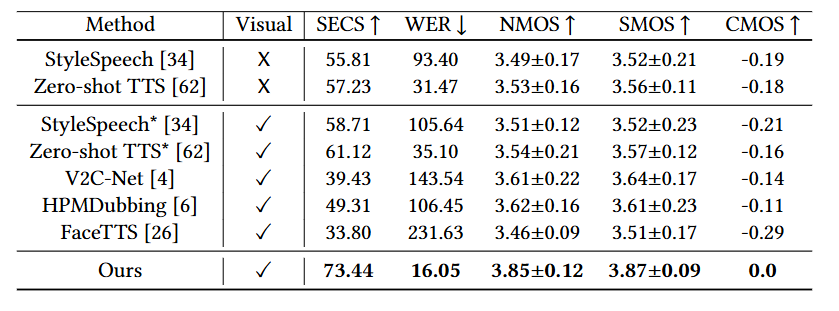
\includegraphics[width=\linewidth]{figs/table4.png} % Replace with the image path for subjective evaluation results
        \caption{Subjective Evaluation Results}
        \label{fig:subjective}
    \end{figure}
\end{columns}
\end{itemize}
\end{frame}


% \begin{frame}
% \frametitle{Experimental Results: Qualitative Analysis of Mel Spectrograms}
% \begin{figure}
% \centering
% 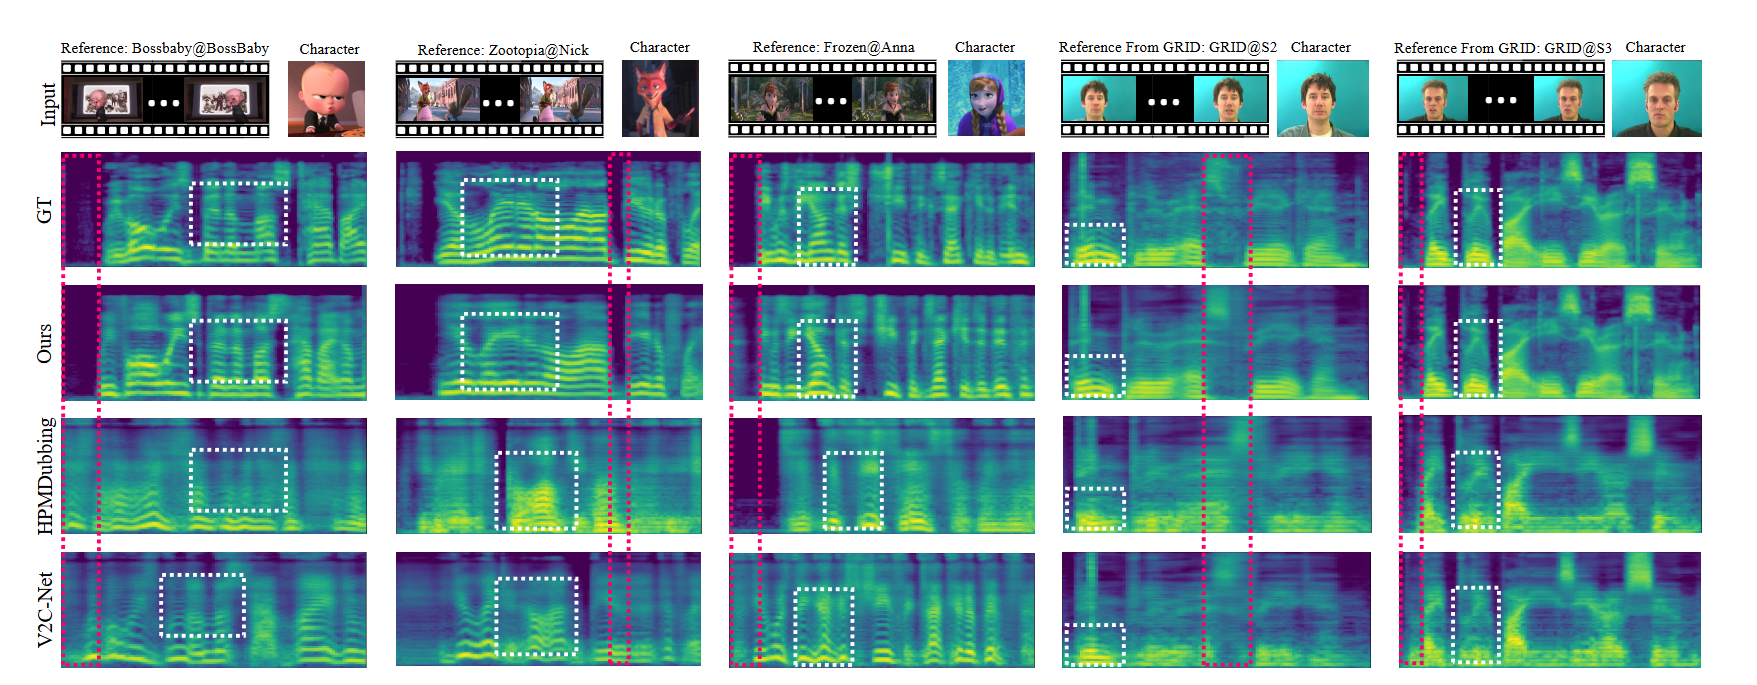
\includegraphics[width=0.6\textwidth]{figs/analysis.png} % Image path
% \caption{Comparison of Mel Spectrograms of Audio Generated by Different Models}
% \end{figure}

% \begin{itemize}
% \item \textbf{Mel Spectrogram Analysis Results:}
%     \begin{itemize}
%     \item \textcolor{red}{Red Box in Figure}: Our model outperforms others in maintaining phoneme and pause durations, especially in the V2C-Animation benchmark with complex speaking speed variations.
%     \item \textcolor{red}{White Box in Figure}: The dubbing generated by our model exhibits clearer and more natural pronunciation details, as evidenced by the clearer spectrum lines.
%     \end{itemize}
% \end{itemize}
% \end{frame}
\begin{frame}
\frametitle{Experimental Results: Qualitative Analysis of Mel Spectrograms}
\begin{figure}
\centering
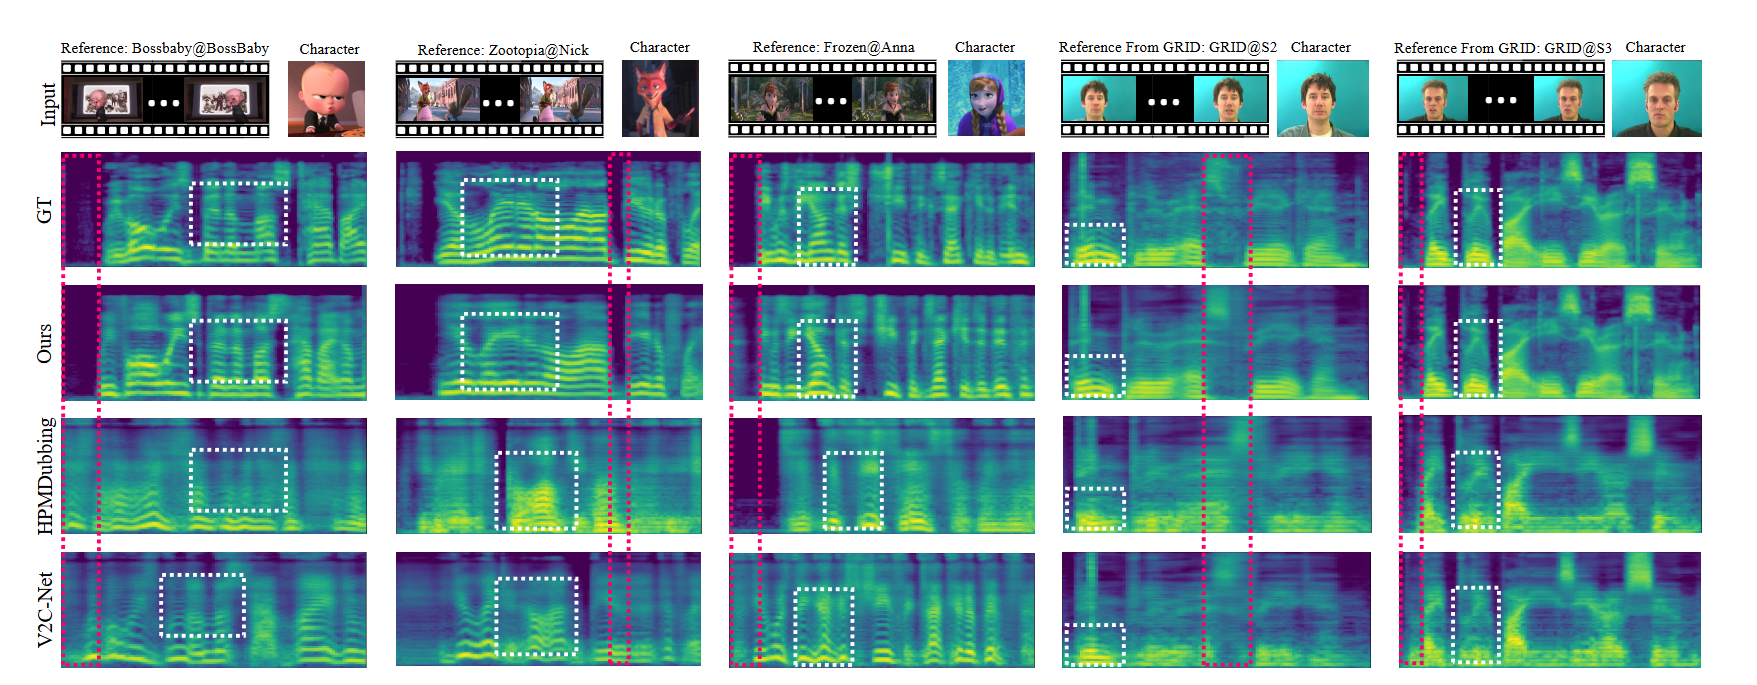
\includegraphics[width=0.6\textwidth]{figs/analysis.png} % Image path
\caption{Comparison of Mel Spectrograms of Audio Generated by Different Models}
\end{figure}

\begin{itemize}
\item \textbf{Analysis Results:}
    \begin{itemize}
    \item \textcolor{red}{Red Box}: the model better maintains phoneme and pause durations, especially in V2C-Animation benchmark.
    \item \textcolor{red}{White Box}: the model shows clearer and more natural pronunciation details.
    \end{itemize}
\end{itemize}
\end{frame}


% \begin{frame}
% \frametitle{Experimental Results: Ablation Study}
% The ablation study results fully demonstrate the necessity of each module.

% \begin{figure}
% \centering
% 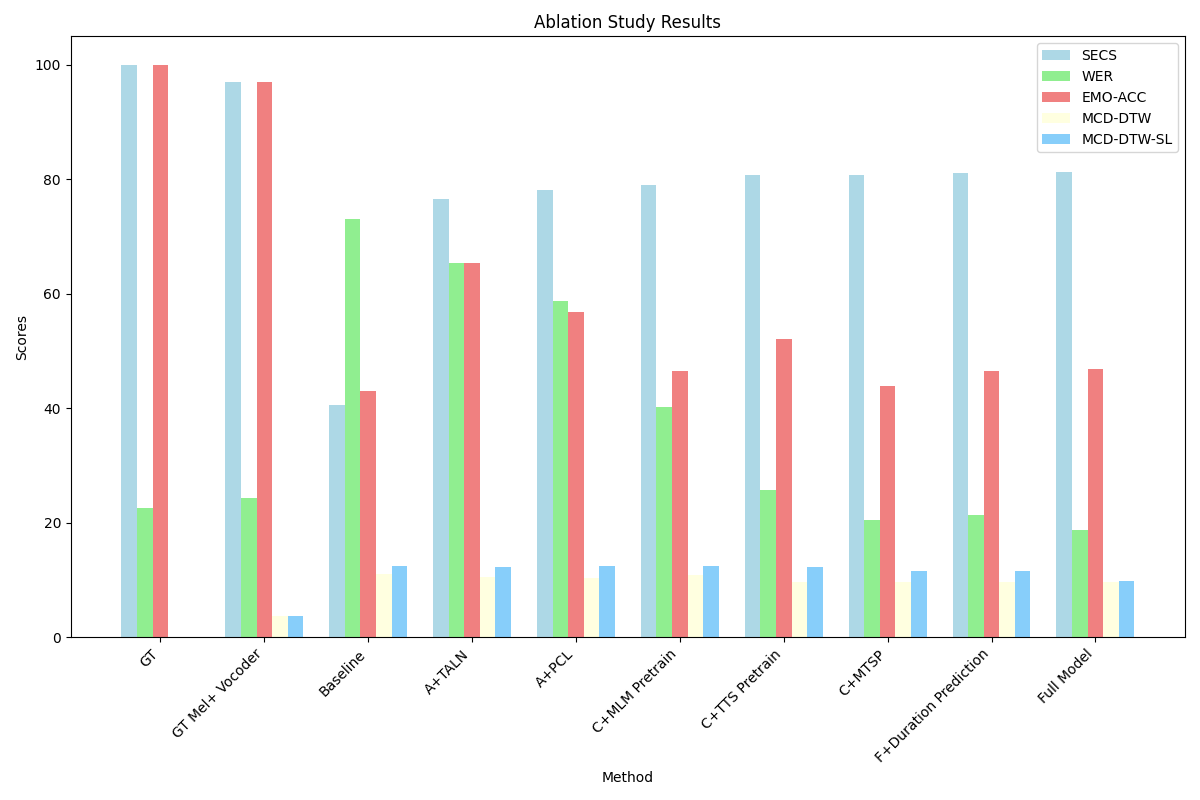
\includegraphics[width=0.4\textwidth]{figs/消融实验.png} 
% \caption{Comparison of Ablation Study Results}
% \end{figure}

% \begin{itemize}
% \item \textbf{PCL Module:} Enhances timbre cloning and emotional consistency.

% \item \textbf{MTSP Module:} Significantly reduces Word Error Rate (WER) and improves pronunciation quality.

% \item \textbf{DCR Module:} Reduces MCD-DTW-SL and enhances duration consistency.

% \end{itemize}
% \end{frame}

\begin{frame}
\frametitle{Experimental Results: Ablation Study}
The ablation study results fully demonstrate the necessity of each module.

\begin{figure}
\centering
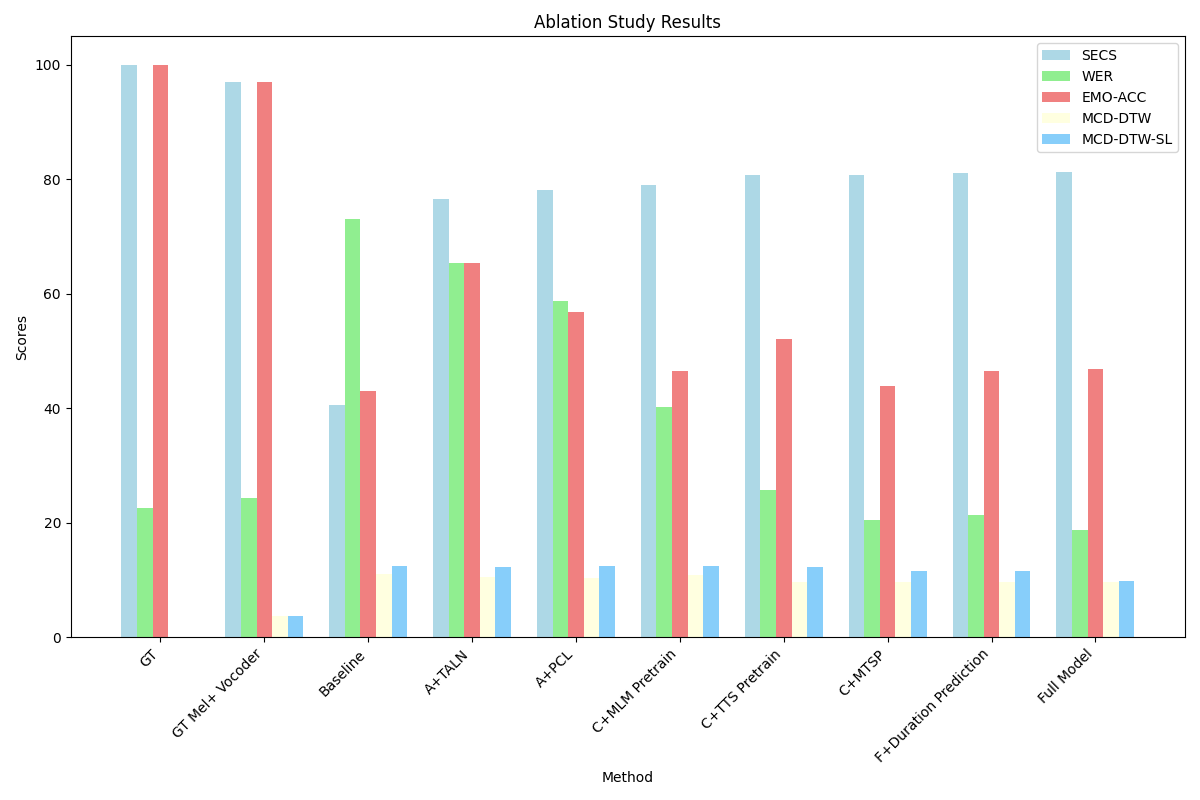
\includegraphics[width=0.4\textwidth]{figs/消融实验.png} 
\caption{Comparison of Ablation Study Results}
\end{figure}

\begin{itemize}
\item \textbf{PCL Module:} Enhances timbre cloning and emotional consistency.
\item \textbf{MTSP Module:} Reduces WER, improves pronunciation quality.
\item \textbf{DCR Module:} Reduces MCD-DTW-SL, enhances duration consistency.
\end{itemize}
\end{frame}
\section{Summary}

% \begin{frame}{Summary of the Paper}
% \begin{itemize}
%     \item \textbf{Research Contributions}:
%     \begin{itemize}
%         \item Proposed a two-stage movie dubbing method that significantly enhances the consistency in timbre, emotional expression, and duration alignment of dubbing through multi-task pre-training and dubbing training.
%         \item The Prosody Consistency Learning (PCL) module improves emotional consistency in dubbing by aligning emotional features with phoneme-level prosody attributes.
%         \item The Duration Consistency Reasoning (DCR) module achieves precise duration matching between dubbing and video by aligning lip motion features with phoneme features.
%     \end{itemize}
%     \item \textbf{Technical Innovations}:
%     \begin{itemize}
%         \item Multi-Task Speaker Pre-training (MTSP) integrates Text-to-Speech (TTS) and Masked Language Model (MLM) tasks, significantly enhancing the model's pronunciation quality and contextual understanding.
%         \item Introduced Timbre-Adaptive Layer Normalization (TALN), which integrates timbre features into phoneme encoding and mel-spectrogram generation by predicting gain and bias for the input vector sequence, ensuring timbre consistency.
%     \end{itemize}
%     \item \textbf{Experimental Results}:
%     \begin{itemize}
%         \item The method outperforms current state-of-the-art methods on multiple metrics across the V2C-Animation and GRID benchmark datasets.
%     \end{itemize}
% \end{itemize}
% \end{frame}
\begin{frame}{Summary of the Paper}
\begin{itemize}
    \item \textbf{Research Contributions}:
    \begin{itemize}
        \item Proposed a two-stage movie dubbing method enhancing timbre, emotion, and duration alignment via MTSP and dubbing training.
        \item PCL module improves emotional consistency by aligning emotions with phoneme-level prosody.
        \item DCR module achieves precise duration matching by aligning lip motion with phoneme features.
    \end{itemize}
    \item \textbf{Technical Innovations}:
    \begin{itemize}
        \item MTSP integrates TTS and MLM tasks, improving pronunciation quality and contextual understanding.
        \item TALN integrates timbre features into phoneme encoding and mel-spectrogram generation, ensuring timbre consistency.
    \end{itemize}
    \item \textbf{Experimental Results}:
    \begin{itemize}
        \item Method outperforms state-of-the-art methods on V2C-Animation and GRID datasets.
    \end{itemize}
\end{itemize}
\end{frame}
% Second page: Reflections on the paper
% \begin{frame}{Reflections on the Paper}
% \begin{itemize}
%     \item \textbf{Learning Method from 'Simple' to 'Complex'}:
%     \begin{itemize}
%         \item The paper employs a two-stage learning framework of "from baby to dubber." It first pre-trains on a large-scale text-to-speech dataset to teach the model clear pronunciation and then fine-tunes on movie dubbing data to adapt to emotional and lip-sync alignment.
%         \item This method effectively addresses the scarcity and complexity of movie dubbing data, significantly improving dubbing quality and consistency.
%     \end{itemize}
%     \item \textbf{Implications for Practical Applications}:
%     \begin{itemize}
%         \item Offers new ideas for data scarcity issues: pre-training on general data followed by fine-tuning on specialized data can enhance model performance.
%         \item Provides insights for multimodal alignment tasks, such as virtual anchors and intelligent customer service.
%     \end{itemize}
%     \item \textbf{Future Research Directions}:
%     \begin{itemize}
%         \item Optimize the two-stage learning framework, such as introducing more modalities like gestures and facial expressions during the pre-training phase.
%         \item Introduce user feedback mechanisms in model training to further optimize dubbing effects.
%     \end{itemize}
% \end{itemize}
% \end{frame}
\begin{frame}{Reflections on the Paper}
\begin{itemize}
    \item \textbf{Learning Method from 'Simple' to 'Complex'}:
    \begin{itemize}
        \item Uses a two-stage framework: pre-trains on TTS data for clear pronunciation, then fine-tunes on dubbing data for emotion and lip-sync alignment.
        \item Addresses data scarcity and complexity, improving dubbing quality.
    \end{itemize}
    \item \textbf{Implications for Practical Applications}:
    \begin{itemize}
        \item Pre-training on general data followed by fine-tuning on specialized data enhances model performance.
        \item Provides insights for multimodal alignment tasks like virtual anchors and customer service.
    \end{itemize}
    \item \textbf{Future Research Directions}:
    \begin{itemize}
        \item Optimize two-stage learning by adding more modalities (e.g., gestures, facial expressions) during pre-training.
        \item Introduce user feedback mechanisms to further optimize dubbing effects.
    \end{itemize}
\end{itemize}
\end{frame}
\begin{frame}
\begin{itemize}
    \item References:
\end{itemize}
    \scriptsize
    \bibliography{ref}
    % % If there are too many references, you can adjust the font size as follows:
    % \tiny\bibliographystyle{apalike}
\end{frame}

\begin{frame}
    \begin{center}
        {\Huge\calligra Thanks!} \\
        \vspace{1cm} % Add some vertical space
    \end{center}
\end{frame}
\end{document}